\documentclass[11pt,a4paper]{report}
\usepackage[utf8]{inputenc}
\usepackage{dirtree}
\setlength{\parindent}{0pt}
\addtolength{\hoffset}{-1cm}
\addtolength{\textwidth}{2cm}
\usepackage{fontspec}
\usepackage{amsmath}
\usepackage{amsfonts}
\usepackage{xcolor,graphicx}
\usepackage[hidelinks]{hyperref}
\usepackage{float}
\usepackage{longtable}
\title{PocketHepia}

\usepackage{chngcntr}
\counterwithout{figure}{chapter}

\usepackage[titletoc,title]{appendix}

\setcounter{secnumdepth}{5}
\usepackage[nonumberlist]{glossaries}
\makeglossaries
%%TODO convert this to english
%%TODO add RFID, add JWT, add SDK, add JS, add JSON, add BSON, add API, add PWA, add REST, add EPFL
%%TODO use all these acronyms in text
\newglossaryentry{nfc}
{
	name=NFC,
	description={est un acronyme pour Near Field Communication qui représente un ensemble de protocoles de communication permettant de communiquer à des distances de quelques centimètres en utilisant l'induction électromagnétique}
}

\newglossaryentry{JVM}
{
	name=JVM,
	description={est un acronyme pour Java Virtual Machine. Il s'agit d'une machine virtuelle permettant d'executer un programme compilé en bytecode Java sur un ordinateur ou un terminal mobile. On parle de langage fonctionnant sur la JVM lorsque la compilation du langage produit du bytecode Java.}
}

\newglossaryentry{IDE}
{
	name=IDE,
	description={est un acronyme pour Integrated Development Environment. Il s'agit d'un programme intégrant un éditeur de texte avec coloration syntaxique et autocomplétion du code pour un ou plusieurs langages de programmation ainsi que des fonctions de compilation, débogage et tout autre fonctionnalité permettant de faciliter et fluidifier le travail du développeur}
}

\usepackage[section]{minted}
\definecolor{mintedbackground}{rgb}{0.95,0.95,0.95}
\usemintedstyle{colorful}

\newmintedfile[javacode]{java}{
breaklines,
bgcolor=mintedbackground,
linenos=true,
numberblanklines=true,
numbersep=5pt,
gobble=0,
frame=leftline,
framerule=0.4pt,
framesep=2mm,
funcnamehighlighting=true,
tabsize=2,
obeytabs=false,
mathescape=false
samepage=true, %with this setting you can force the list to appear on the same page
showspaces=false,
showtabs =false,
texcl=false,
}

\newmintedfile[jsoncode]{json}{
breaklines,
bgcolor=mintedbackground,
linenos=true,
numberblanklines=true,
numbersep=5pt,
gobble=0,
frame=leftline,
framerule=0.4pt,
framesep=2mm,
funcnamehighlighting=true,
tabsize=2,
obeytabs=false,
mathescape=false
samepage=true,
showspaces=false,
showtabs =false,
texcl=false,
}

\newmintedfile[kotlincode]{kotlin}{
breaklines,
bgcolor=mintedbackground,
linenos=true,
numberblanklines=true,
numbersep=5pt,
gobble=0,
frame=leftline,
framerule=0.4pt,
framesep=2mm,
funcnamehighlighting=true,
tabsize=2,
obeytabs=false,
mathescape=false
samepage=true,
showspaces=false,
showtabs =false,
texcl=false,
}

\newmintedfile[jscode]{javascript}{
breaklines,
bgcolor=mintedbackground,
linenos=true,
numberblanklines=true,
numbersep=5pt,
gobble=0,
frame=leftline,
framerule=0.4pt,
framesep=2mm,
funcnamehighlighting=true,
tabsize=2,
obeytabs=false,
mathescape=false
samepage=true,
showspaces=false,
showtabs =false,
texcl=false,
}

\newmintedfile[tscode]{typescript}{
breaklines,
bgcolor=mintedbackground,
linenos=true,
numberblanklines=true,
numbersep=5pt,
gobble=0,
frame=leftline,
framerule=0.4pt,
framesep=2mm,
funcnamehighlighting=true,
tabsize=2,
obeytabs=false,
mathescape=false
samepage=true,
showspaces=false,
showtabs =false,
texcl=false,
}

\newmintedfile[xmlcode]{xml}{
breaklines,
bgcolor=mintedbackground,
linenos=true,
numberblanklines=true,
numbersep=5pt,
gobble=0,
frame=leftline,
framerule=0.4pt,
framesep=2mm,
funcnamehighlighting=true,
tabsize=2,
obeytabs=false,
mathescape=false
samepage=true,
showspaces=false,
showtabs =false,
texcl=false,
}


\begin{document}
\begin{titlepage}
	\centering
	{\scshape \LARGE ITI Bachelor Project \par}
	\vspace{1cm}
	{\scshape\Large August 2018\par}
	\vspace{1.5cm}
	{\huge\bfseries PocketHepia\\A student card platform based on NFC \par}
	\vspace{2cm}
	{\Large\itshape Maxime Alexandre Lovino\par}
	\vfill
	Supervised by\par
	Prof. Mickaël Hoerdt
	\vfill
		\begin{minipage}{.5\textwidth}
		\centering
		
\includegraphics[width=.7\linewidth]{assets/logo_hepia.png}
	\end{minipage}%
	\begin{minipage}{.5\textwidth}
		\centering
		
\includegraphics[width=.7\linewidth]{assets/logo_hes.png}
	\end{minipage}
\end{titlepage}
\shipout\null
\pagenumbering{roman}
\tableofcontents
\newpage
\listoffigures
\newpage
\chapter*{Acknowledgements}
\glsaddall
\printglossary[title=Terms and Definitions]
\newpage
\shipout\null
\pagenumbering{arabic}
\chapter{Introduction}
Since starting my studies at HEPIA almost three years ago after two years at EPFL, I've been shocked by the lack of commodities and study spaces for students. Some of this lack is due to the difference in scale between the two schools, one of them being composed of mainly three building in a constrained city environment and the other an almost-autonomous campus outside the city. But, actually, there isn't really a lack of space at HEPIA, but a lack of space that students can use to study. Most of the classrooms are locked when not in use by a teacher. When asking about why that is the case, I've been told that it was mainly for security concerns because of the equipment present inside the rooms. If the rooms stayed unlocked, there was no way of knowing who stole or broke something. I suggested the idea of giving access to select students to these classrooms to study and work on projects but it wasn't practical because copies of keys had to be made, the students had to make a money deposit to make sure that they didn't run away with the keys etc.\\ 

The real solution would have been to use our student cards as an electronic door key to access the rooms, as well as enable other uses for the cards, such as using them as electronic wallets to simplify the payments at the canteen during lunch break. When I suggested the idea, people mostly laughed at me and said "[...] they're never going to do it, unless someone actually does it, presents it as a finished product and then they decide to use it." So, here I am, after 3 years studying at HEPIA and for my Bachelor Project I decided to work on this exact idea. A multi-function student card platform built on NFC technology with accompanying mobile and web application for administrators to manage the platform and for students to monitor their usage statistics.

%% TODO %%MH : One solution, plutôt que The Real solution
%%MH : separer la deuxieme partie de phrase "as well" dans une autre phrase
%%MH : => La solution de l'acces aux portes et le porte monnaie sont deux features 
%%MH : separee.

\section{Project inspiration - Camipro EPFL}
\subsection{The card and the official core platform}
The inspiration for this project mainly comes from my experience studying at EPFL. The EPFL student card, named Camipro\cite{camipro:homepage}, contains an RFID chip that allows to perform various tasks that simplify student life on campus. The use cases for the Camipro card are the following:
\begin{itemize}
    \item Electronic wallet to pay at every canteen on campus as well as select third-party retailers (for example the Migros shop present on campus)
    \item Access key to unlock doors and buildings
    \item Card to collect documents sent to the centralised printing pool system at any printer on campus
    \item Rent public bicycles\footnote{All students have access to a free Publibike account on their card \url{https://www.publibike.ch/en/publibike/}} on campus and in the Lausanne area
    \item Rent cars by linking a Mobility\footnote{\url{https://www.mobility.ch/en/}} subscription to the card
    \item Borrow books at the library
    \item Use electric car chargers on campus
    \item Turn on booked electrical barbecues present on campus\footnote{The service PolyGrill allows students to book free barbecues on campus and access them with their camipro \url{https://camipro.epfl.ch/cms/site/camipro/lang/en/polygrill_electric_barbecues}}
\end{itemize}

An accompanying web platform called MyCamipro was built as part of the Camipro launch to manage and activate the different services on the card as well as see the recent transactions and the rooms we were given access to.

\begin{figure}[H]
\begin{center}
	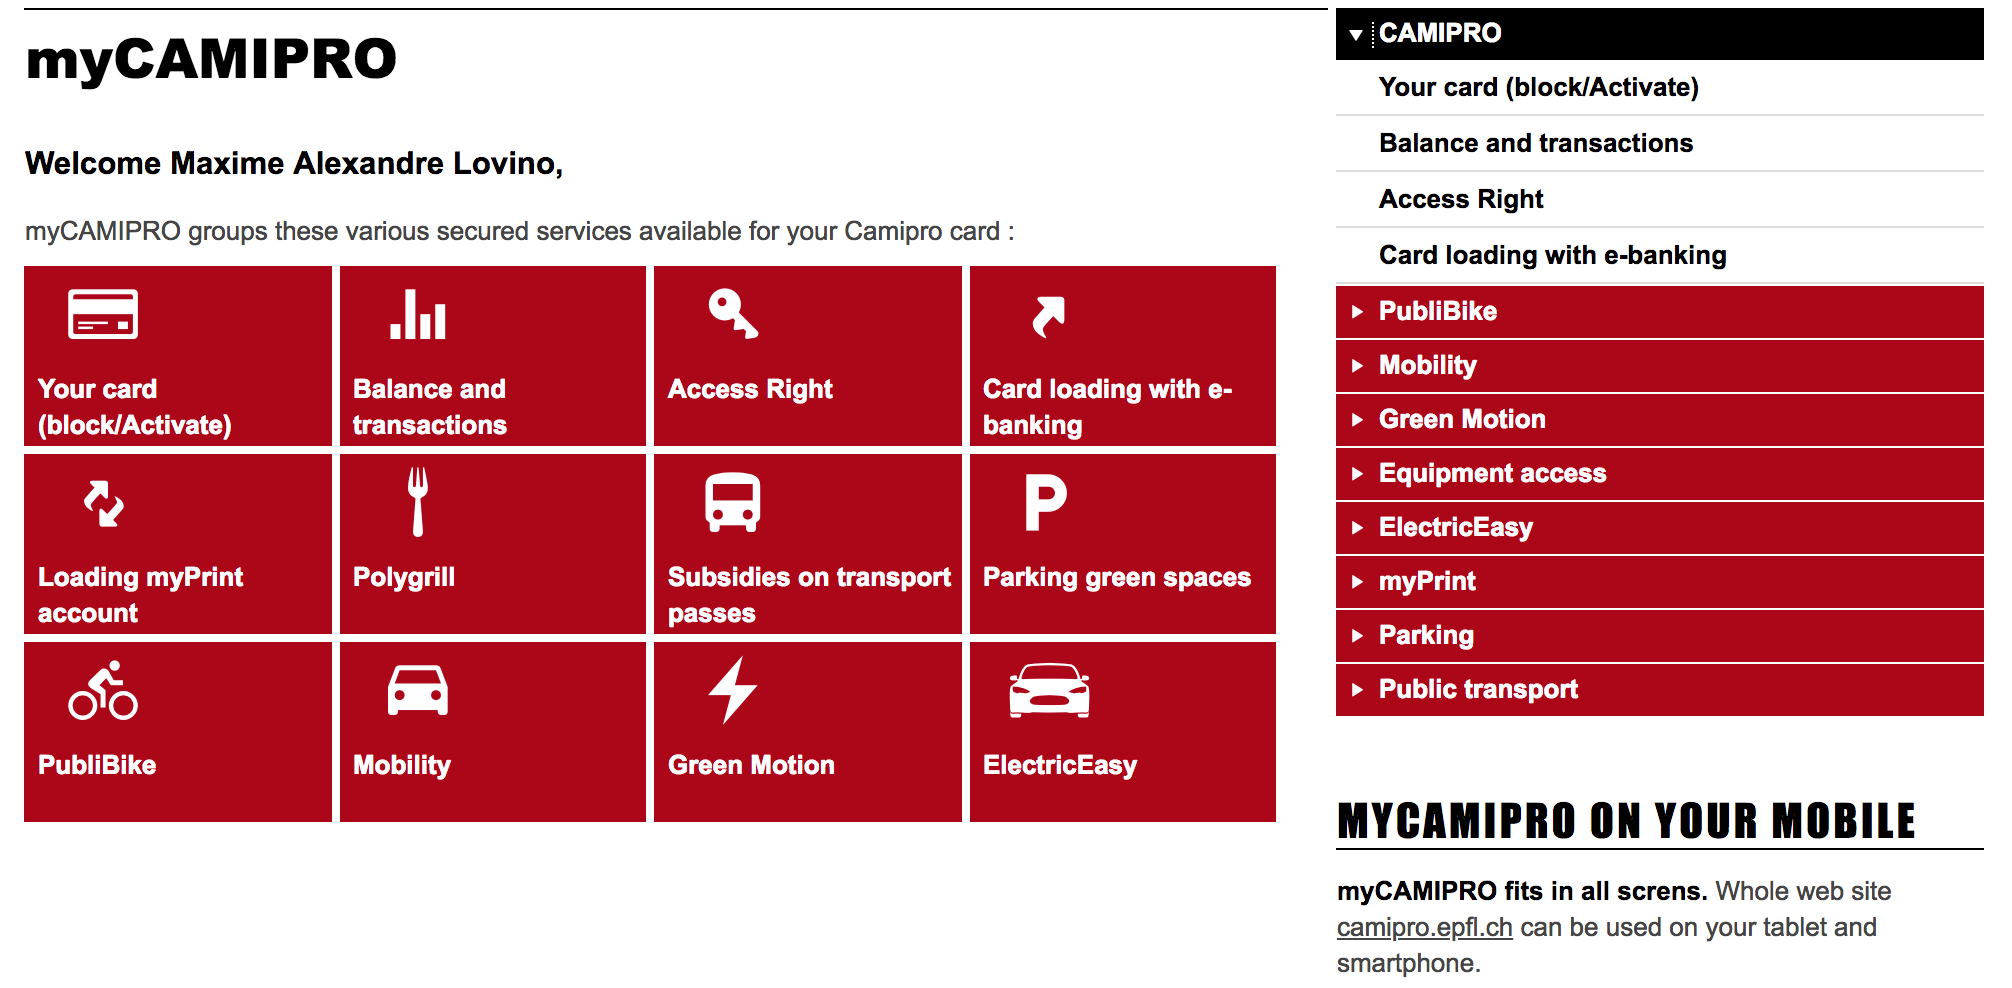
\includegraphics[width=.6\textwidth]{assets/camipro_website.png}
	\caption{Screenshot of the MyCamipro website}
\end{center}
\end{figure}

\subsection{PocketCampus}
With the increased usage of smartphones by students, in 2010 a team of 20 computer science students decided to build the PocketCampus application as part of a software engineering class. They continued working on the project after the academic project was finished and it became the official EPFL application in 2013. \cite{camipro:creation}. \\

Initially you could mainly see the balance of your Camipro card on the app, but version after version, the development team added new integration in the app by collaborating with different services at EPFL.
These functions include:
\begin{itemize}
    \item Accessing the menus of all canteens on campus
    \item Searching through the whole EPFL directory
    \item Having access to IS-Academia data to see course schedule and grades
    \item Printing from your smartphone on the EPFL print system
    \item Accessing Lausanne public transportation itineraries
    \item Accessing Moodle documents
\end{itemize}

After having integrated every requested features, the team launched a beta web version of PocketCampus for EPFL in June 2018. They also started diversifying their business by working on PocketCampus as a platform that can be integrated in other companies and stopped working exclusively with EPFL. They announced plans on partnering with Lausanne University (UNIL) to integrate their platform there.

\begin{figure}[H]
\begin{center}
	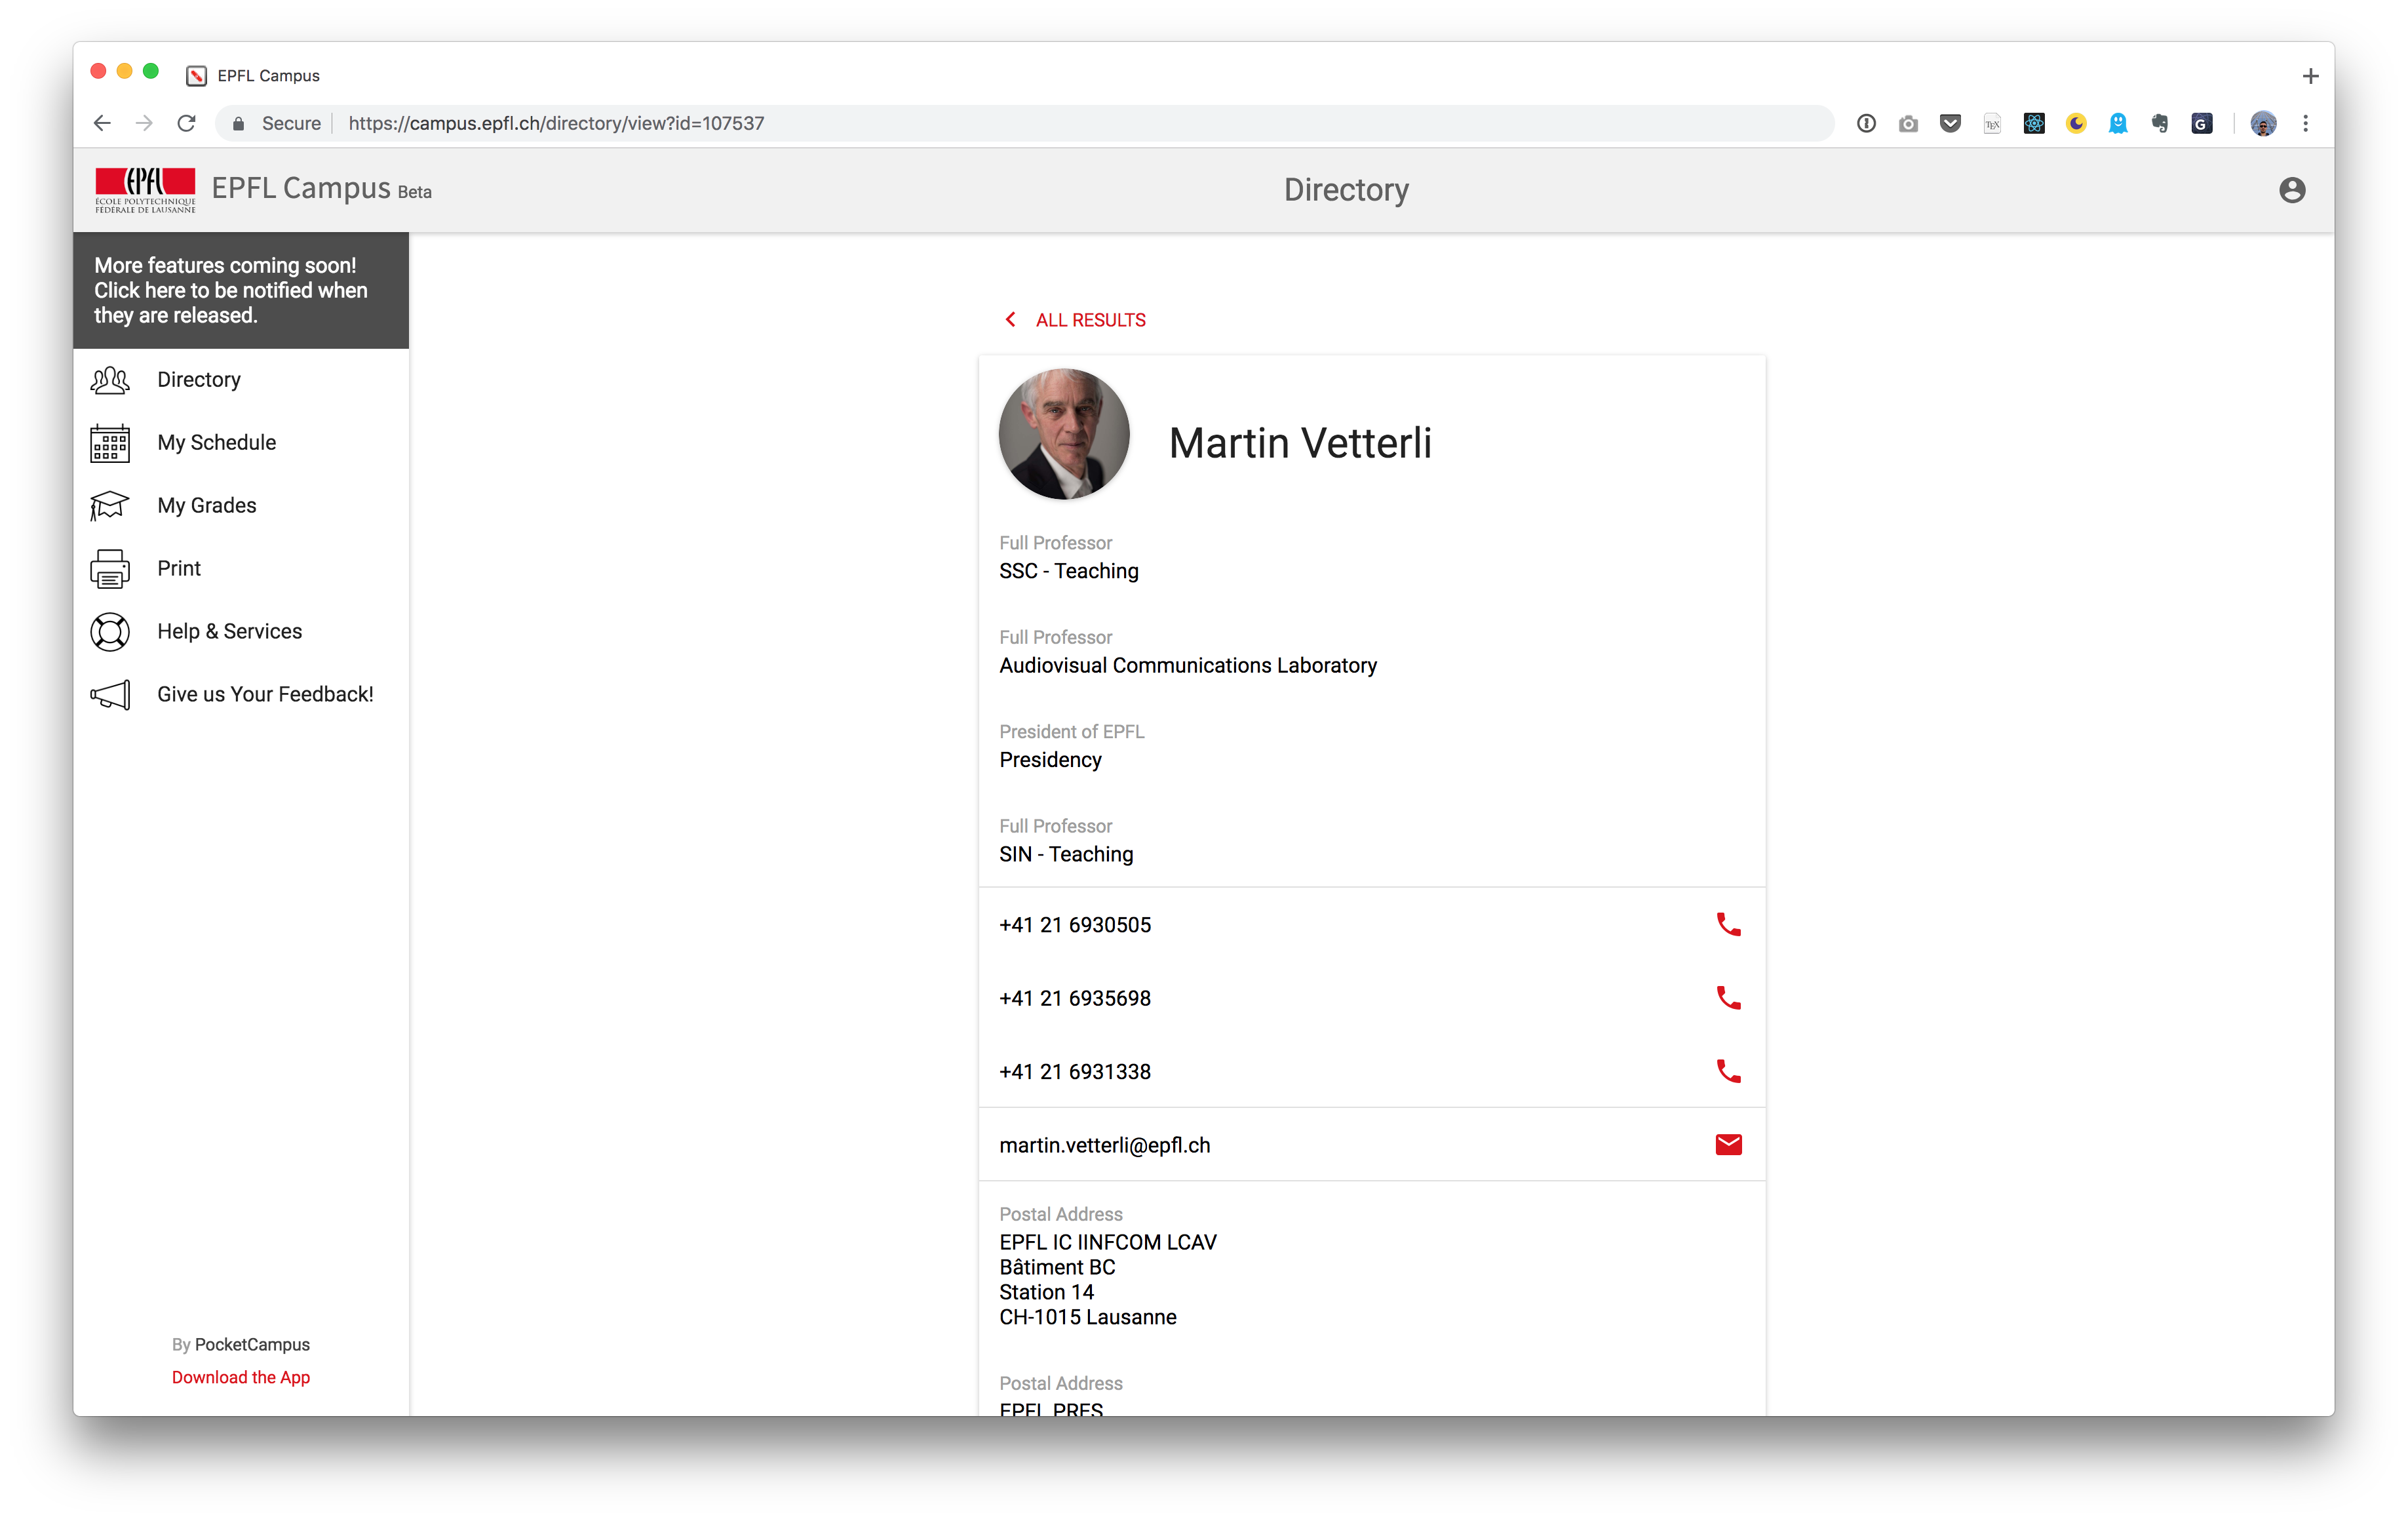
\includegraphics[width=.8\textwidth]{assets/web_pocketcampus.png}
	\caption{Screenshot of the web version of PocketCampus}
\end{center}
\end{figure}
\begin{figure}[H]
\begin{center}
	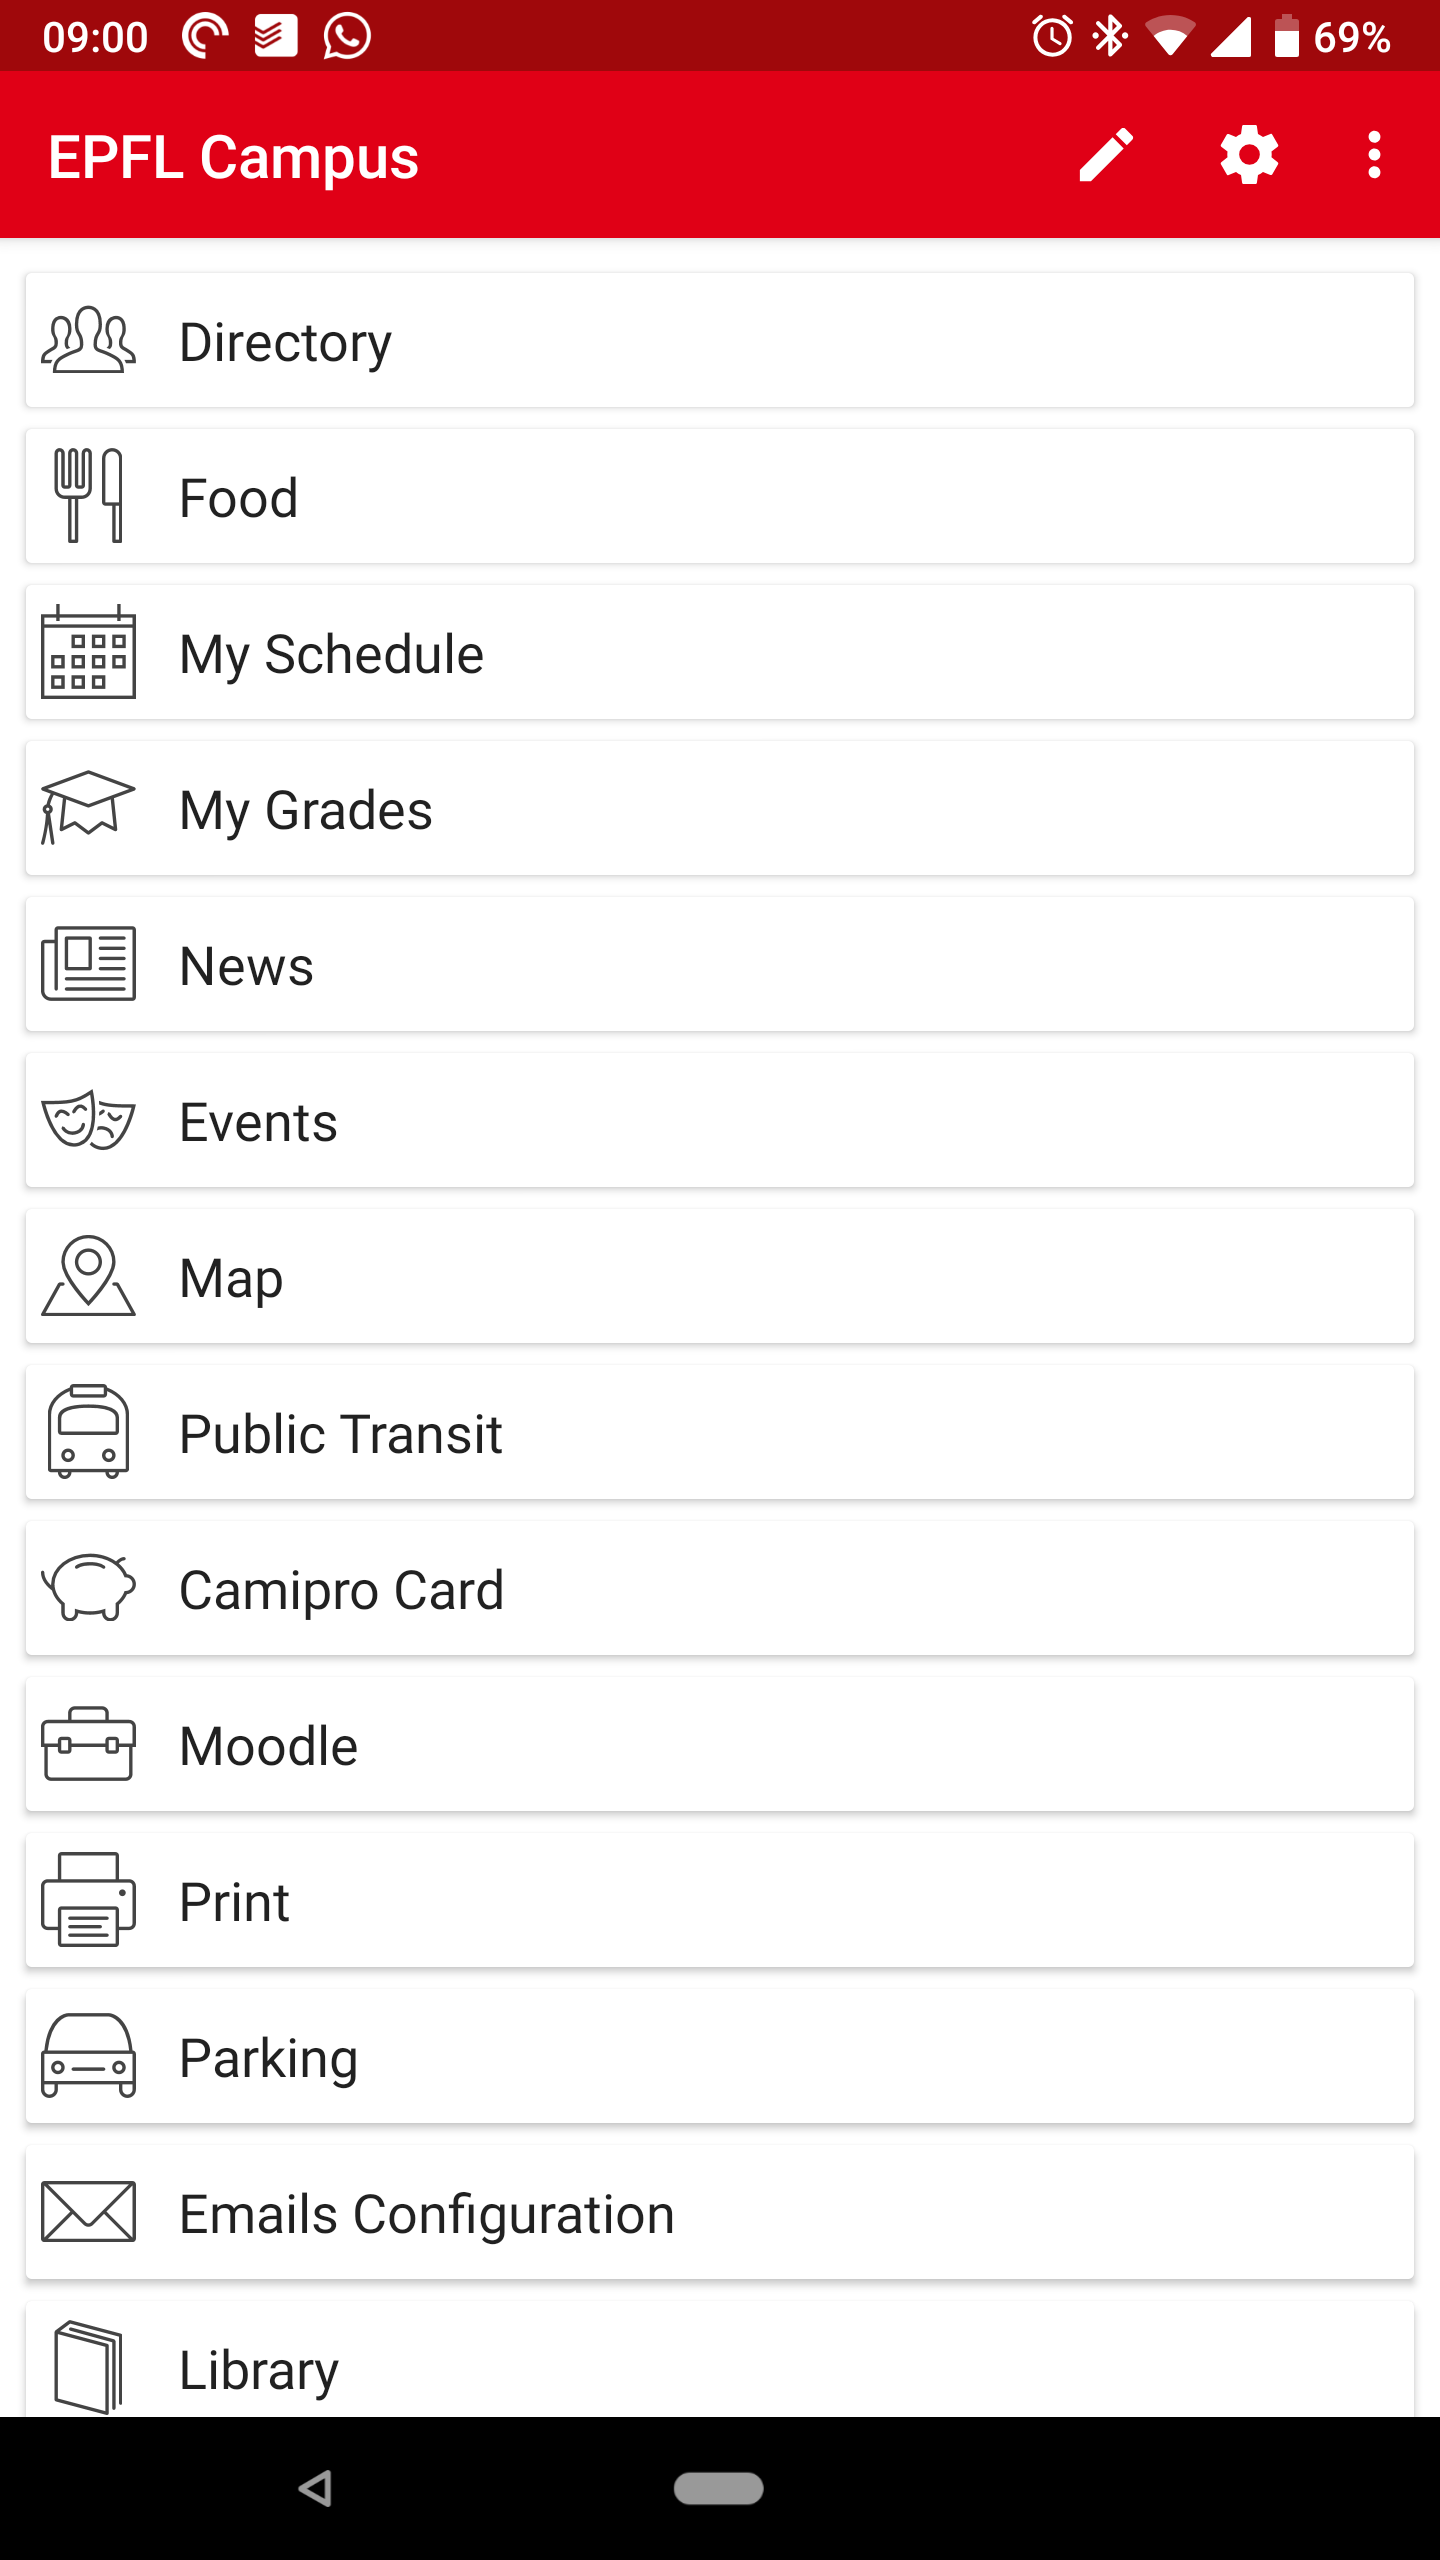
\includegraphics[width=.5\textwidth]{assets/pocketcampus_mobile.png}
	\caption{PocketCampus Android application}
\end{center}
\end{figure}

\chapter{The project}
The project is called PocketHepia, reminiscent of the name of the project at EPFL and will consist of the two parts of the EPFL project presented earlier: the student card platform, as well as the applicative platform to access information.\\


The idea of this project is not to build as many features as the EPFL platform due to the time constraints inherent to the Bachelor Project, but rather to focus on some key aspects of the card at first, namely payments, access control and library. We are also building features on the payment side that are not available on the EPFL platform, for example the ability to send money between users. The project of course will be extensible with other features outside the scope of the Bachelor Project. \\

In this chapter, we will present the main features, roles and user stories for the project as specified at the beginning of this one. All of these are part of the project, but not necessarily part of the Bachelor Project. The idea was to specify the entire project and to start implementing a subset of the functionality for the academic project and continue working on the rest as well as new features outside this scope. Mainly we wanted to remain independent of other school services and infrastructure because of the associated time it would take to get permissions and setup integrations, as well as restrictions to development environments to secure access to these services. For each element of this chapter, we will specify whether it is going to be implemented as part of the Bachelor Project.\\

The project is composed of three main components:
\begin{itemize}
    \item The physical student card
    \item An administration component
    \item An user facing component
\end{itemize}

A mobile application and a web application will be developed and both will offer the same user facing features as well as specific administrative features relevant to each application.

\section{Features of the app}
As stated before, we decided to limit the project to the three most important features in our opinion and, out of these, two are going to be implemented as part of the bachelor project.

\subsection{Payments}

The first feature is the electronic wallet functionality. We decided to start with this one because it would be bring the most benefits to the students and would not need specific hardware or collaboration with any school service. Every user has an electronic wallet linked to its account on the platform and can then send money to any other user by choosing the amount to send and tapping the user's card on his phone. Users can be assigned a specific role (see section \ref{roles_section}) to allow them to receive money directly from a card.\\

There will be two main ways to add money to an user wallet. Either the user can give cash money to a person with administrative role that will then add money to the user's balance. Or the user will be able to add money to its account by using its credit card on the web application.\footnote{At the moment, the project is still in the development phase so no bank accounts have been linked to this project and you will be able to recharge your account only using a specific test credit card generated for development purposes}

\subsection{Accesses}

To continue, the second element of the project is the handling of access control through the platform. This was the original pain point we noticed at HEPIA with the lack of an easy way to handle accesses to the available classrooms. We will be able to create different areas to group rooms inside them. For example, an area could be an entire floor or labs for a specific section of HEPIA.\\

As far as giving access to users, we can give access to a room from a given date and specify if needed an end date for the access. For example, we can setup access for a user until the end of the current semester. We also decided to introduce an optional time range during the day during which the given access is active, so we can for example allow a student to enter a room only between 8am and 7pm. \\

We also specified the ability to delegate the administration of an area to a user, so that access to rooms can be handled at a department or section level in the school for example (see section \ref{roles_section}). This feature is planned but will not be implemented as part of the Bachelor Project.

\subsection{Library books}
\label{books_feature}
Finally, the last feature of the project would be an integration with the library to be able to use the card as a library card. Our approach at first was to think about creating the book loans on our platform with the ISBN to identify the book and integrate with the REST API built for BibApp but it wouldn't have been very effective because the library already handles the loans through the NEBIS platform.\\

The correct way to handle this would be to link the library NEBIS identifier for every user with their account on our platform and then ask NEBIS for API Access to their platform to retrieve book loans for all users and display them on the mobile and web application. This would also benefit people working at the library as they would not need to change their current workflow to accommodate.\\

We don't have the time during the bachelor project to start a discussion with NEBIS to get access to the required information so this feature will have to be implemented later on.
\section{Roles}
\label{roles_section}
We defined a set of roles for the users on the platform. First, every member of the platform is a simple user. This means that the person has an account on the platform, can login to the web and android application and has read access to its payments, its accesses and its other information and can send money to other users.\\

Then, there is the admin role that can be added to an user. This role enables the creation of users, attribution of roles, the consultation of administrative logs as well as the creation of access components (rooms, readers) and the attribution of accesses to users.\\

While these two roles would have been enough to handle all our features. We decided to specify roles specific to different components of the platform.\\

One of these roles is the "Accept payments" role. This is specific to a canteen or a shop that wants to handle payments using the student card. While every user can send money to another user from the mobile app by tapping the other user's card, this isn't very practical for a canteen or a shop where the transactions should go the other way around. So the shop creates the payment and taps the user's card to take money from it. At first, we wanted this feature to be available to everyone but we thought about security concerns with this solution because a student could create a payment from the app and start tapping his phone on lost cards or even on people's pocket and if the card was detected it would "steal" their money. So by enabling this feature as a role, we could only allow trusted people, such as canteen's owners to receive payments in that way. \\

Furthermore, due to the introduction of GDPR recently, we created a specific role called "Auditor" to access sensitive logs concerning all users, mainly access logs and transaction history. Only a user with this role can view all transactions between users and access logs for every room.\\
%%TODO add reference for GDPR and footnote to explain why

Then, there are two roles that will not be implemented as part of the Bachelor project, the "Can invite" and "Area admin" role. The first is to allow specific users to create temporary accounts without needing to contact an administrator. A use case for this would be a teacher creating a temporary account for a visiting colleague from another school. The "Area admin" role consists of delegating the administration of the accesses for an area to an user. Similar to the concept of DNS zones delegation, an administrator could for example give this role to the ITI section dean to allow him to give access to the rooms present on his floor.\\

Finally, the last role is the "Librarian" role that as its name implies is attributed to users working for the library. This role enables the creation of books loans at the library for users. As stated in section \ref{books_feature}, this role will certainly be removed completely because there is already a system in place to handle book loans at the library.

\section{The models}
%%TODO Add global relational database schema with multiplicities (UML)
\subsection{User Accounts}
\begin{figure}[H]
\begin{center}
	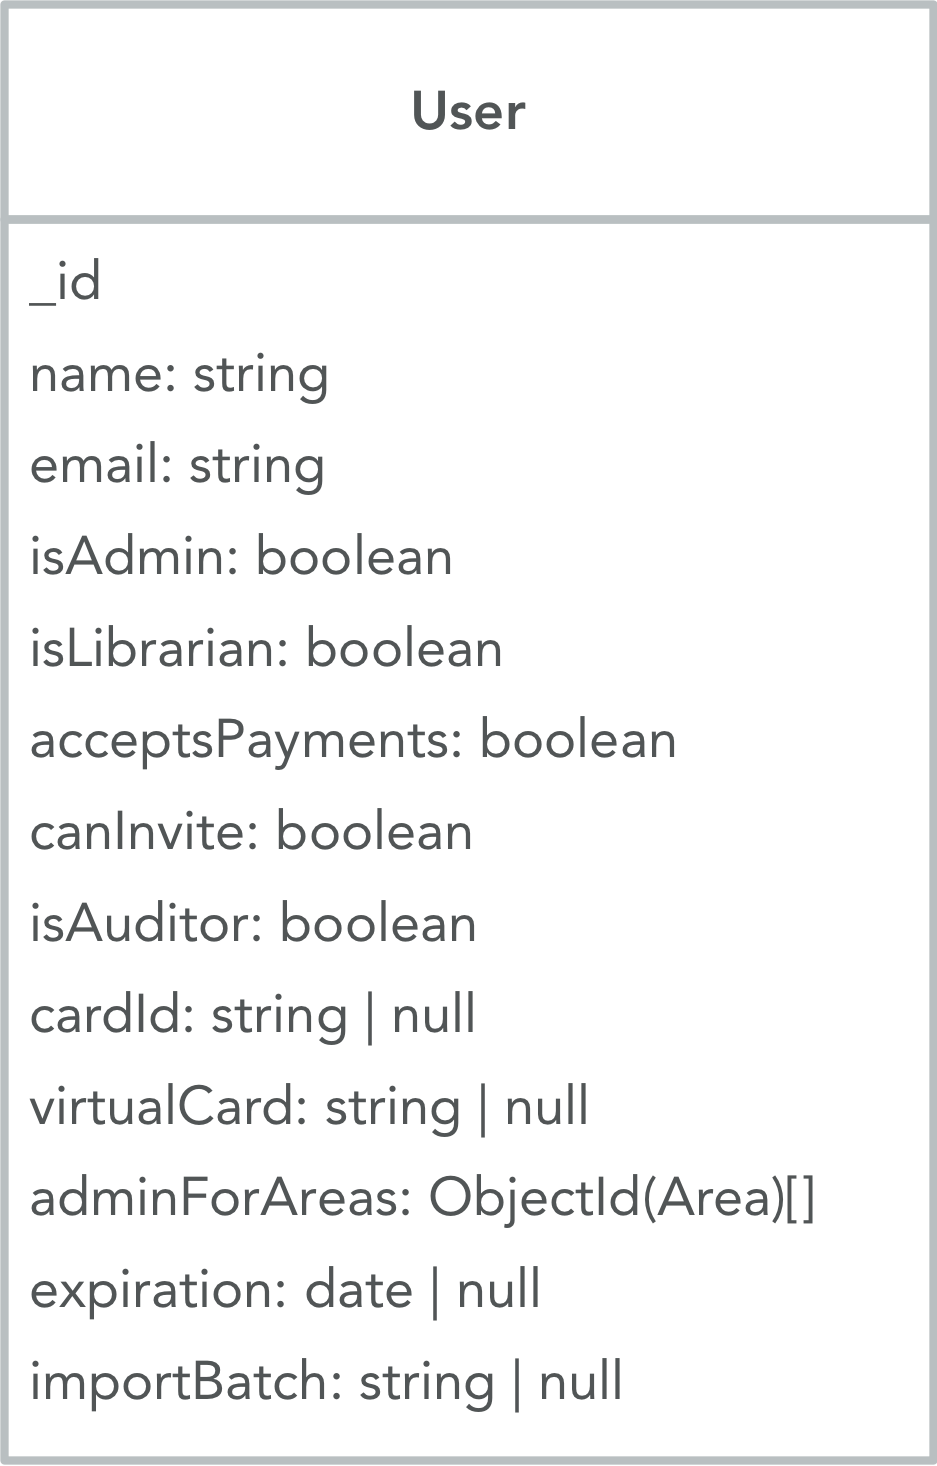
\includegraphics[width=.4\textwidth]{assets/user_model}
	\caption{User Model}
\end{center}
\end{figure}

The first of our models is the User. A user collection is created to store all users on the platform. Users are identified by their email address and will login with their email and password, their full name is also stored. The authentication specific fields will be added to the model by Passport.JS (see section \ref{technological choices}). A boolean field is also stored for each permission.\\

The expiration date, the virtual card and the delegation of admin zones are not implemented as part of this bachelor project. \\

Finally, the \verb+importBatch+ is set if the user is imported with a CSV file so that we can group all users imported together and undo the import if necessary.
\subsubsection{Integration with existing AAI user accounts}
If this project is put in production at HEPIA, we will have to only change this model to integrate it with an existing authentication service, such as AAI or with a directory LDAP service.\\

In that case, we would remove information already present in the authentication service such as name and email and just store the unique identifier from the authentication service in our model. This model would act as an augmented database on top of the existing service. We would then forward all login/password authentication request to the authentication service and would create the entry for the user in our database after the first login.\\

This is inspired by the way Nextcloud\footnote{\url{https://nextcloud.com/}} for example stores user accounts that are linked to a directory service, for example an Active Directory. It stores the full Distinguished Name from the directory service as the unique identifier for the account to link the local account to the directory account.\\

While we could have asked Switch-AAI to integrate AAI authentication in our application, the time constraints of the project were too tight to launch a discussion and we wanted to stay independent of other services in this phase to avoid being slowed down by for example needing to run our servers on the HEPIA network exclusively to access the directory.
\subsection{Payments}
\begin{figure}[H]
\begin{center}
	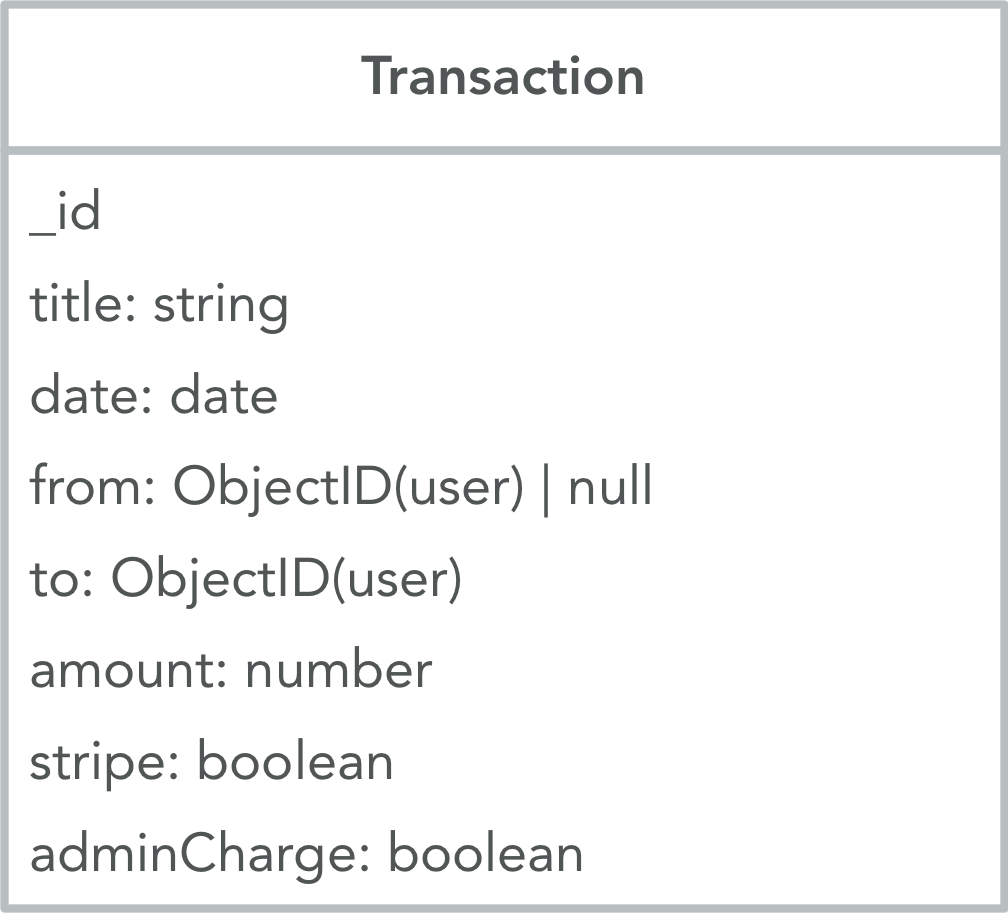
\includegraphics[width=.4\textwidth]{assets/transaction_model}
	\caption{Transaction Model}
\end{center}
\end{figure}
To handle payments, we defined a Transaction model that represents a money transaction. We store the id of the \verb+to+ and \verb+from+ users instead of embedding the users document inside the transaction in order to avoid using too much space in the database. The number of transactions can grow very high and it is a waste of space to store two full user documents in each transaction\footnote{For more on that, see section \ref{mongo_references} on Mongo References}. Finally, we handle the two type of recharges for the user account by setting the \verb+from+ user to \verb+null+ because the money does not come from any user account and set the corresponding \verb+stripe+ or \verb+adminCharge+ field to true. \\

The balance of a user is calculated from the list of transactions in which the user takes part. It is calculated as the sum of the transactions in which the user is the beneficiary minus the sum of transactions in which he makes the payment.
\subsection{Accesses}
\begin{figure}[H]
\begin{center}
	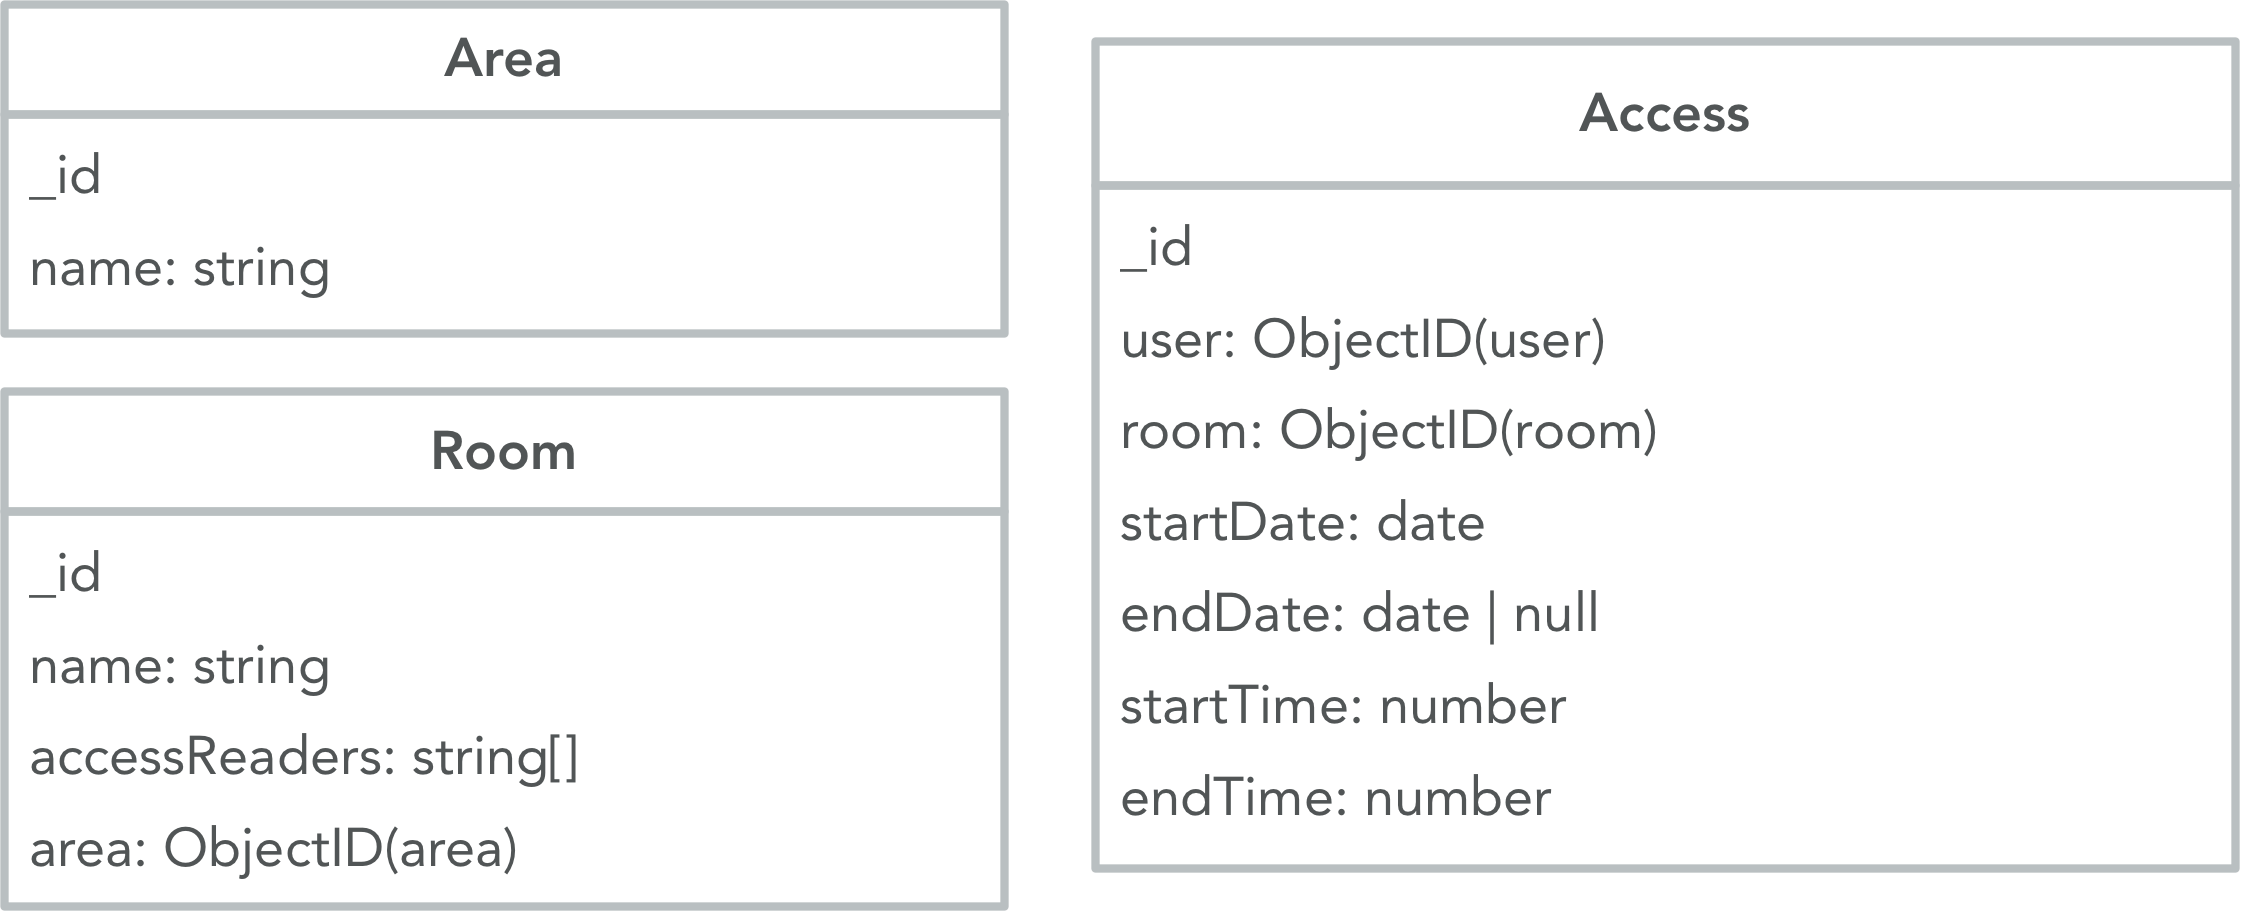
\includegraphics[width=.8\textwidth]{assets/access_model}
	\caption{The three models handling accesses}
\end{center}
\end{figure}

The access part of PocketHepia is composed of three models. We defined Areas, Rooms and Accesses. An area contains multiple rooms and each room has a specific set of accesses. Similarly to the payments model, we reference from the child to the parent with the ID of the parent. The room has the id of the area it is part of, and the access stores the id of the user and the room. \\

When deleting an area, we delete all rooms contained in that area. When deleting a room, we delete all accesses associated with the room. This is done using Mongoose hooks (see section \ref{mongoose_hooks}) to ensure that on every removal, we cascade it through the children.
\subsubsection{Access requests}
%%TODO talk about this and not implementing them
\subsubsection{Access logs}
%%TODO talk about this and not implementing them
\subsection{Logs}
\begin{figure}[H]
\begin{center}
	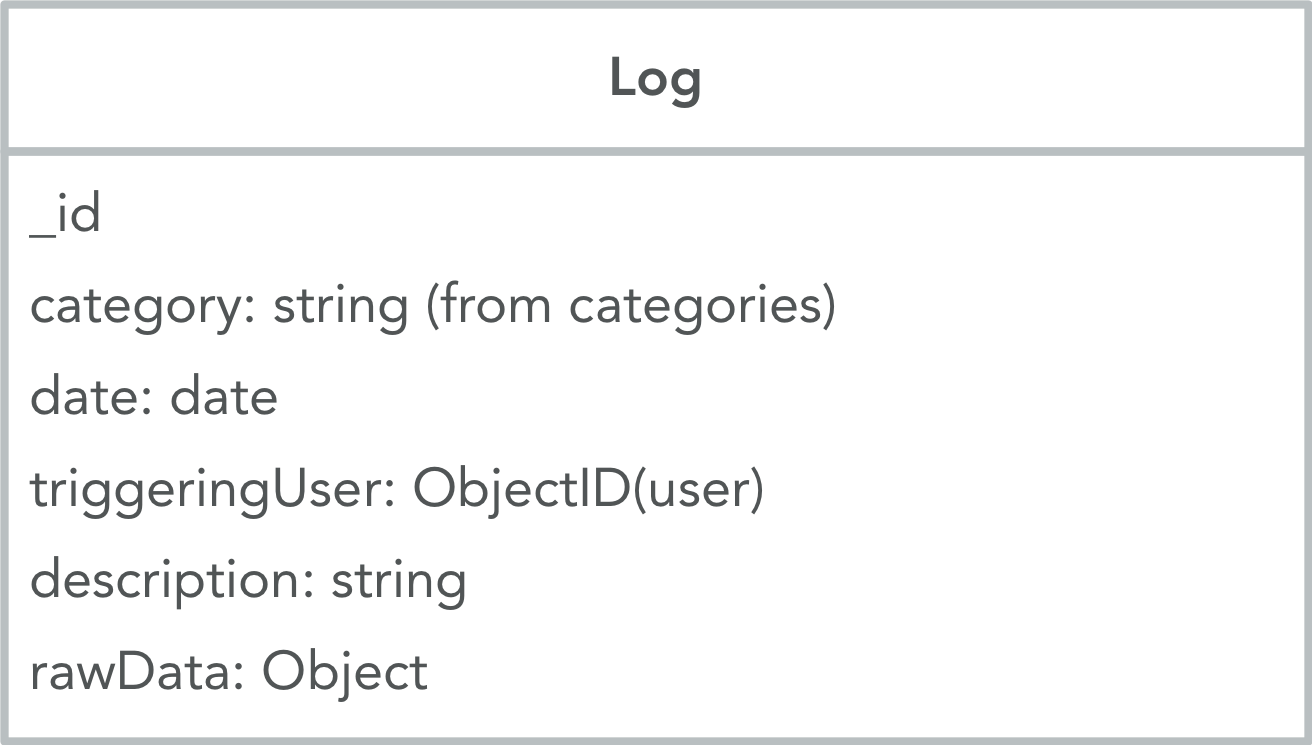
\includegraphics[width=.6\textwidth]{assets/log_model}
	\caption{Log Model}
\end{center}
\end{figure}
Finally, we decided to log all administrative actions and make the logs visible to all admins on the website. Giving access to a room or creating a new account can be sensitive, so we have to keep an historic of those actions.\\

We defined a Log model to store the logs in the DB and several log categories to distinguish the different logs and filter them.

The log categories are:
\begin{itemize}
\item User creation
\item User changes its password
\item User deleted
\item Admin imports users
\item Admin cancels an import
\item Admin assigns a NFC Tag
\item Admin removes a NFC Tag
\item Admin adds money to a user balance
\item Admin resets a user password
\item Admin changes a user permissions
\item Admin creates an area
\item Admin deletes an area
\item Admin creates a room
\item Admin deletes a room
\item Admin gives an access
\item Admin removes an access
\end{itemize}
As well as categories for features we will not implement yet:
\begin{itemize}
\item Admin delegates an area
\item Admin removes an area delegation
\item Admin completes an access request
\item Admin deletes an access request
\end{itemize}

The category for a log entry is stored as a \verb+string+ and we setup validation on the model to ensure the \verb+string+ used corresponds to a category.\\

We also store an embedded object we call \verb+rawData+, this allows us to store additional information specific to each category. For example for a permission change, we store the user before and after the changes. \\

Finally, the field \verb+triggeringUser+ stores the id of the user that did the action, we can then filter the logs to find out everything a specific person did.
\section{User stories}
From the beginning, we wrote simple user stories as a roadmap for the project features we wanted to implement. All of these features are not part of this academic project but are part of the broader student card project. 
%% TODO Continue text, references the table
%% TODO talk about features implemented during the summer, they will be explained in the report how to implement them and then implemented outside the project for the demo

\renewcommand*{\arraystretch}{1.5}
\begin{longtable}[c]{|p{0.33\linewidth}|l|p{0.33\linewidth}|}
\hline
\textbf{User story name}                                                                                                                       & \textbf{Priority} & \textbf{Status as of July 11th 2018}                \\ \hline
\endhead
%
User must be able to login using username and password (then using JWT to communicate with backend)                                            & 1 - Essential     & Done                                             \\ \hline
Admin can create users from the website                                                                                                        & 1 - Essential     & Done                                             \\ \hline
User can view its total balance and a summary of its information on the homepage (web and application)                                         & 2 - Important     & Done                                             \\ \hline
User can view all its transactions on the transactions page (web and application)                                                              & 2 - Important     & Done                                             \\ \hline
User can view its total balance on the transactions page (web and application)                                                                 & 2 - Important     & Done                                             \\ \hline
User can view all its accesses to rooms on the access page (web and application)                                                               & 2 - Important     & Done                                             \\ \hline
Admin can delete users from the website                                                                                                        & 2 - Important     & Done                                             \\ \hline
Admin can reset password for all users from the website                                                                                        & 2 - Important     & Done                                             \\ \hline
Admin can create users in batch by importing a CSV file                                                                                        & 2 - Important     & Done                                             \\ \hline
Admin can create areas from the website                                                                                                        & 2 - Important     & Done                                             \\ \hline
Admin can create rooms from the website                                                                                                        & 2 - Important     & Done                                             \\ \hline
Admin can give access to a room for a user from the website (start/end date and timerange)                                                     & 2 - Important     & Done                                             \\ \hline
Admin can remove an access from the website                                                                                                    & 2 - Important     & Done                                             \\ \hline
Admin can view all accesses for a user                                                                                                         & 2 - Important     & Done                                             \\ \hline
Admin can view all accesses for a room                                                                                                         & 2 - Important     & Done                                             \\ \hline
Admin can assign a physical card to a user from the Android app                                                                                & 2 - Important     & Done                                             \\ \hline
Admin can remove a physical card for a user from the Android app                                                                               & 2 - Important     & Done                                             \\ \hline
Admin can view all administrative logs from the website and filter them                                                                        & 2 - Important     & Done                                             \\ \hline
All administrative actions should be logged                                                                                                    & 2 - Important     & In progress (all implemented actions are logged) \\ \hline
User having the “Accept Payment” permission can create a payment from the Android app and scan a user card to validate the payment             & 2 - Important     & Done                                             \\ \hline
User can change its password                                                                                                                   & 3 - Normal        & Done                                             \\ \hline
User can send money to another user from the Android app                                                                                       & 3 - Normal        & Done                                             \\ \hline
Admin can undo a user batch import                                                                                                             & 3 - Normal        & Done                                             \\ \hline
Admin can delete areas from the website                                                                                                        & 3 - Normal        & Done                                             \\ \hline
Admin can delete rooms from the website                                                                                                        & 3 - Normal        & Done                                             \\ \hline
Admin can change permissions of users from the website                                                                                         & 3 - Normal        & Done                                             \\ \hline
Admin can add money to a user account                                                                                                          & 3 - Normal        & Done                                             \\ \hline
User can view all its borrowed books on the books page                                                                                         & 4- Nice to have   & Not started                                      \\ \hline
All accesses should be logged                                                                                                                  & 4- Nice to have   & Not started                                      \\ \hline
User can add money to its account using its credit card (using Stripe)                                                                         & 4- Nice to have   & Frontend in progress                             \\ \hline
User can create a virtual card from the application and use it                                                                                 & 4- Nice to have   & Placeholder and navigation on Android only       \\ \hline
User can request access to a room from the website                                                                                             & 4- Nice to have   & Not started                                      \\ \hline
Admin can delegate admin rights for an area to a user                                                                                          & 4- Nice to have   & Not started                                      \\ \hline
Admin can view and mark as done room access requests                                                                                           & 4- Nice to have   & Not started                                      \\ \hline
Auditor should be able to view access logs                                                                                                     & 4- Nice to have   & Not started                                      \\ \hline
Auditor should be able to view all payments logs                                                                                               & 4- Nice to have   & Not started                                      \\ \hline
User having the “can invite” permission can create a temporary user from the Android app and the website                                       & 4- Nice to have   & Not started                                      \\ \hline
User having admin rights for an area can give access to an user to a room in that area (start/end date and start/end hour)                     & 4- Nice to have   & Not started                                      \\ \hline
User having admin rights for an area can view and mark as done room access requests for that area                                              & 4- Nice to have   & Not started                                      \\ \hline
Onboarding setup process in web frontend to create first user when no users exists in the DB                                                   & 4- Nice to have   & Not started                                      \\ \hline
Ability to connect to LDAP (Active Directory for example) for users and authentication                                                         & 4- Nice to have   & Not started                                      \\ \hline
Librarian can create a loan for a book for a user from the Android app                                                                         & 5 - Not relevant  & Removed                                          \\ \hline
Librarian can view current bookings for all users from the website and Android app and mark the borrowing as Complete (all history on website) & 5 - Not relevant  & Removed                                          \\ \hline
\caption{User stories}
\label{user_stories_table}\\
%%TODO sort the table by priority
\end{longtable}


\section{Technological choices}
\label{technological choices}
\subsection{The data and backend}
%%TODO talk about JWT
For the data and backend part of the project, we decided to build a unique backend for both the web and mobile clients. We would need a database to store the data of our models and a service to access to access that data. The easier solution would be to build a REST API in front of a database. To do this, we saw two main possibilities: a PHP REST API coupled with a SQL Database or a Node.JS Express REST API coupled with a Mongo DB. While we could mix these and use a SQL Database with Node.JS, we wanted to use the better affinity possible between the two. With the increase in popularity in Javascript based backends, we decided to rule out the PHP option and keep the Express/Mongo option. This is also due to the fact that PHP feels dated and does not provide a clear structure unless you use a PHP Framework to complement it. \\

%%TODO PHP less modern => node js better => why nosql is better => php without frameworks is a mess

The second solution that was suggested was to use an object syncing platform to directly synchronise data with all of our clients. One of these platforms is \emph{Realm Platform\footnote{\url{https://realm.io/products/realm-platform}}} and we decided to study the advantages of it for our project and decide if we should use it over the Express/Mongo option.
%%TODO talk about realm
\subsubsection{Realm vs. Express-MongoDB}
\begin{figure}[H]
\begin{center}
	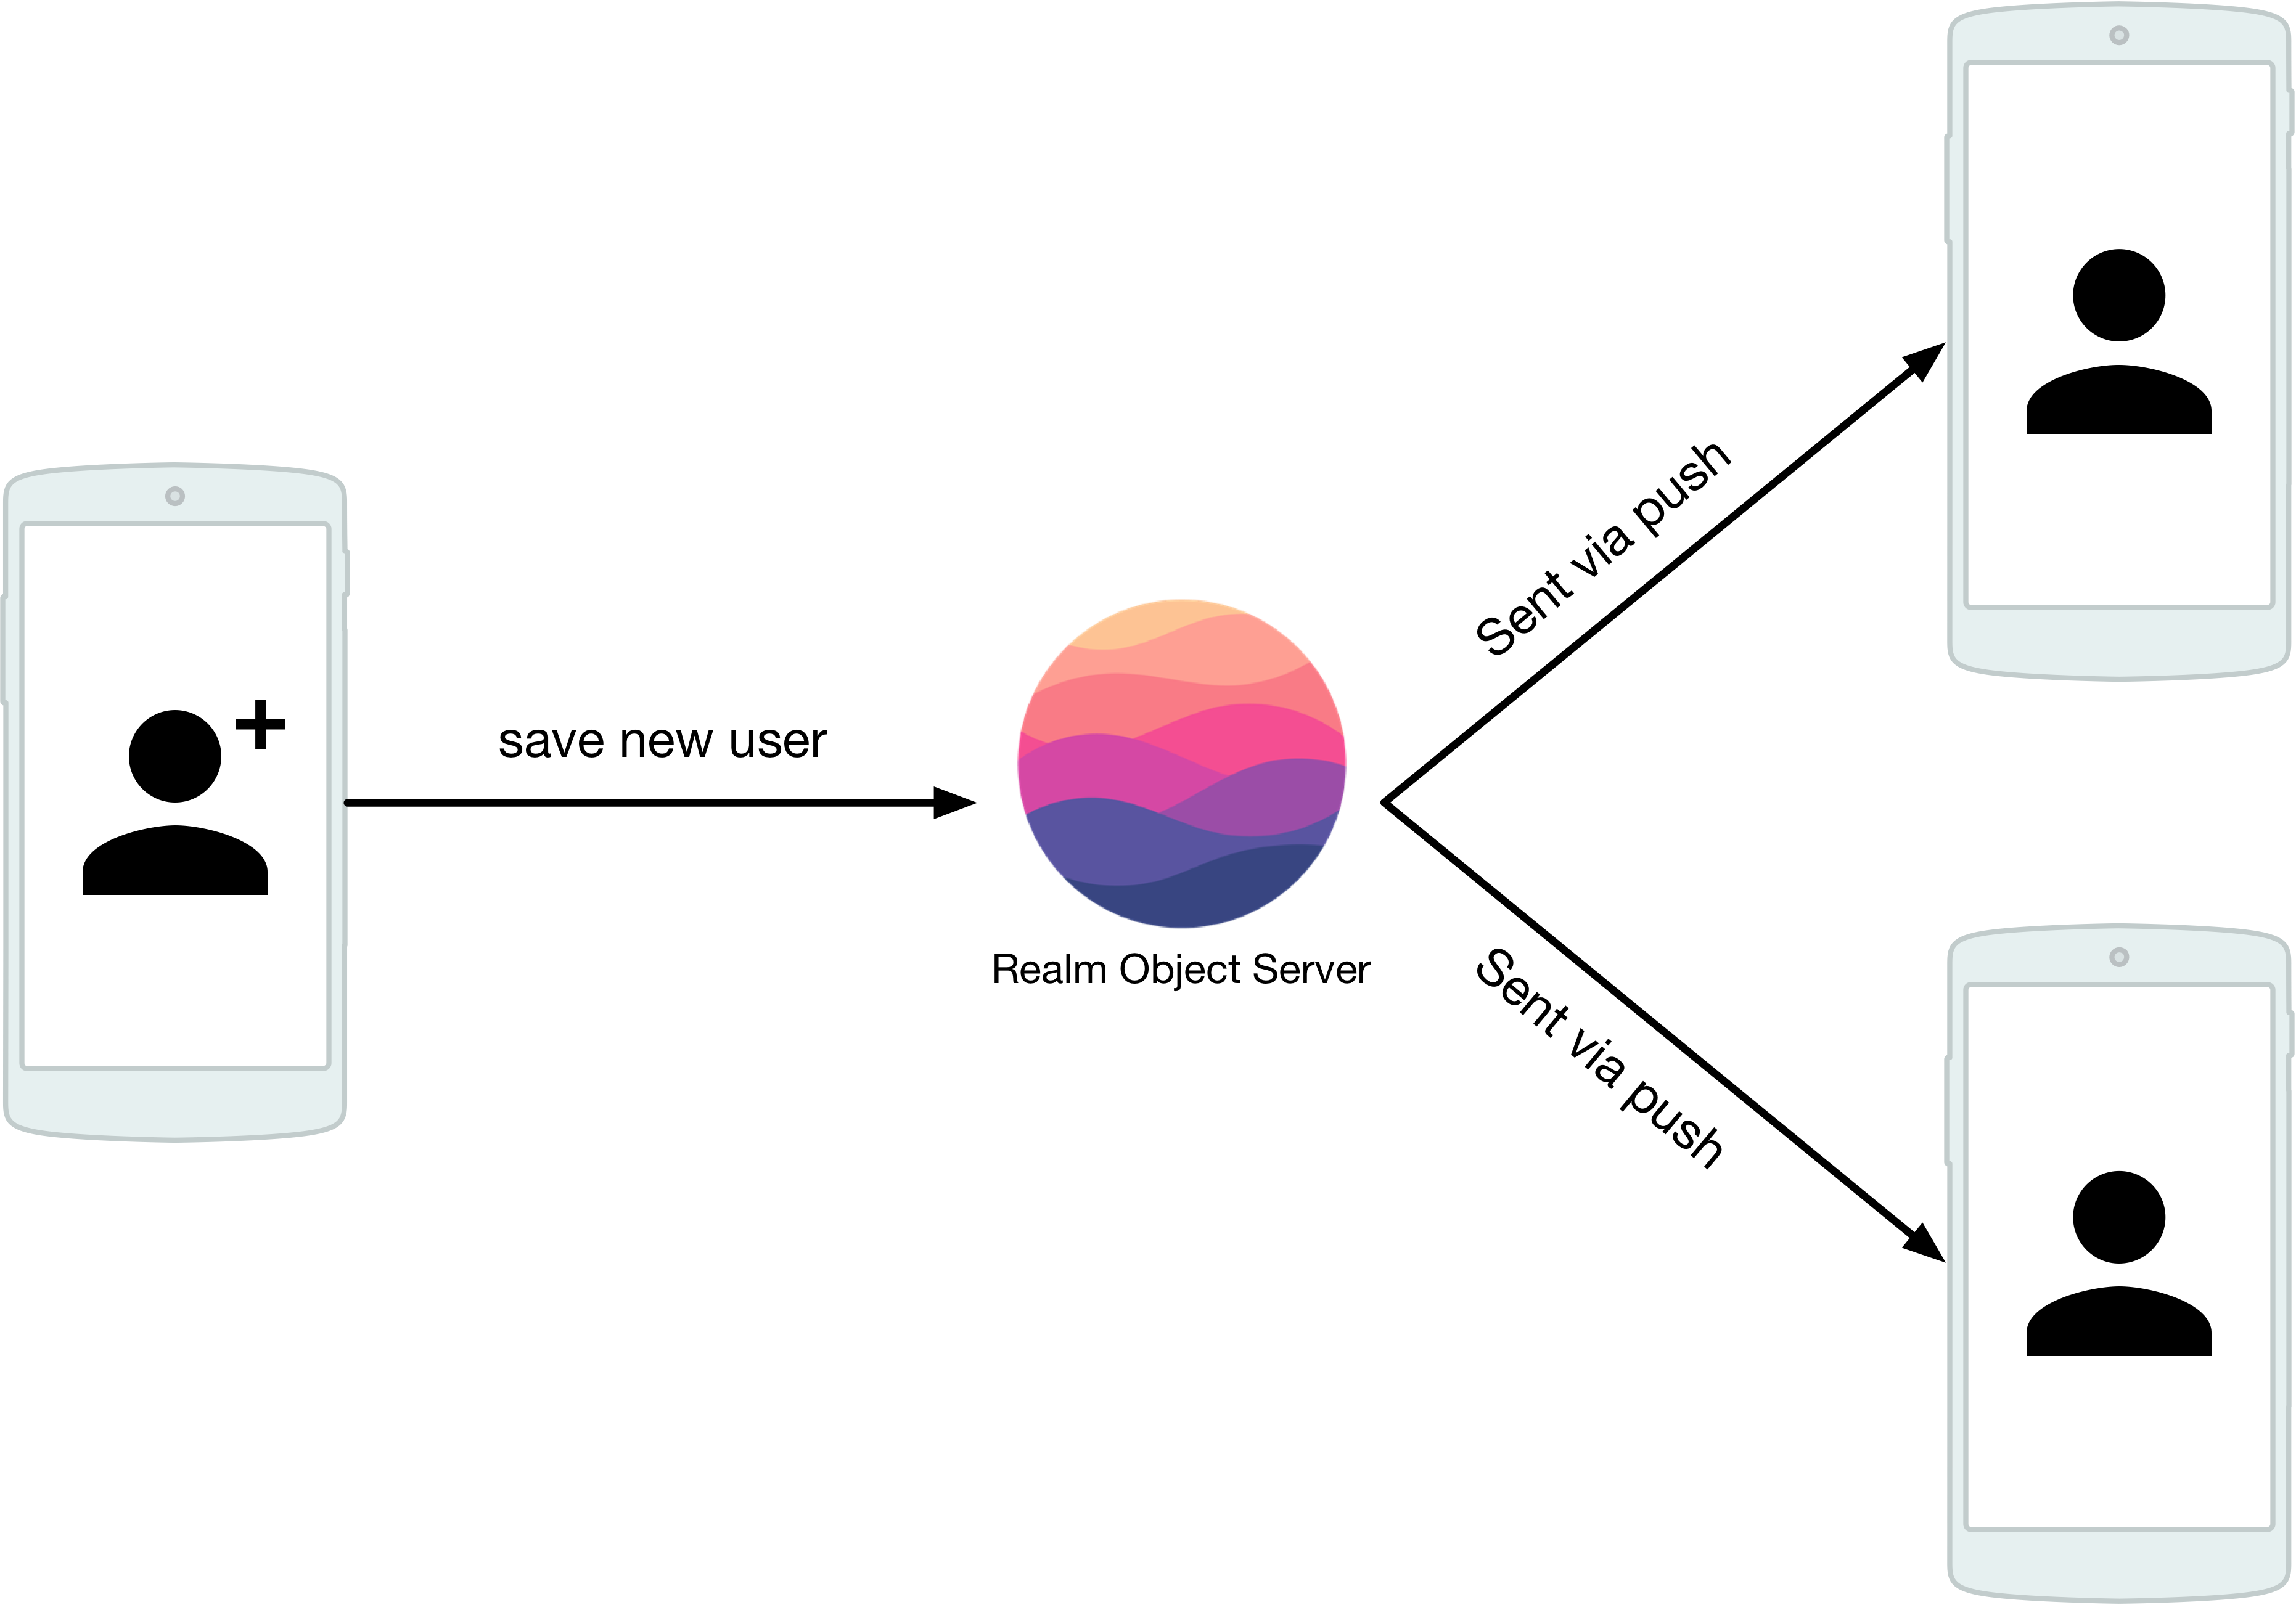
\includegraphics[width=.8\textwidth]{assets/realm_architecture}
	\caption{Saving an object in Realm}
	\label{realm_object_saving_figure}
\end{center}
\end{figure}

\begin{figure}[H]
\begin{center}
	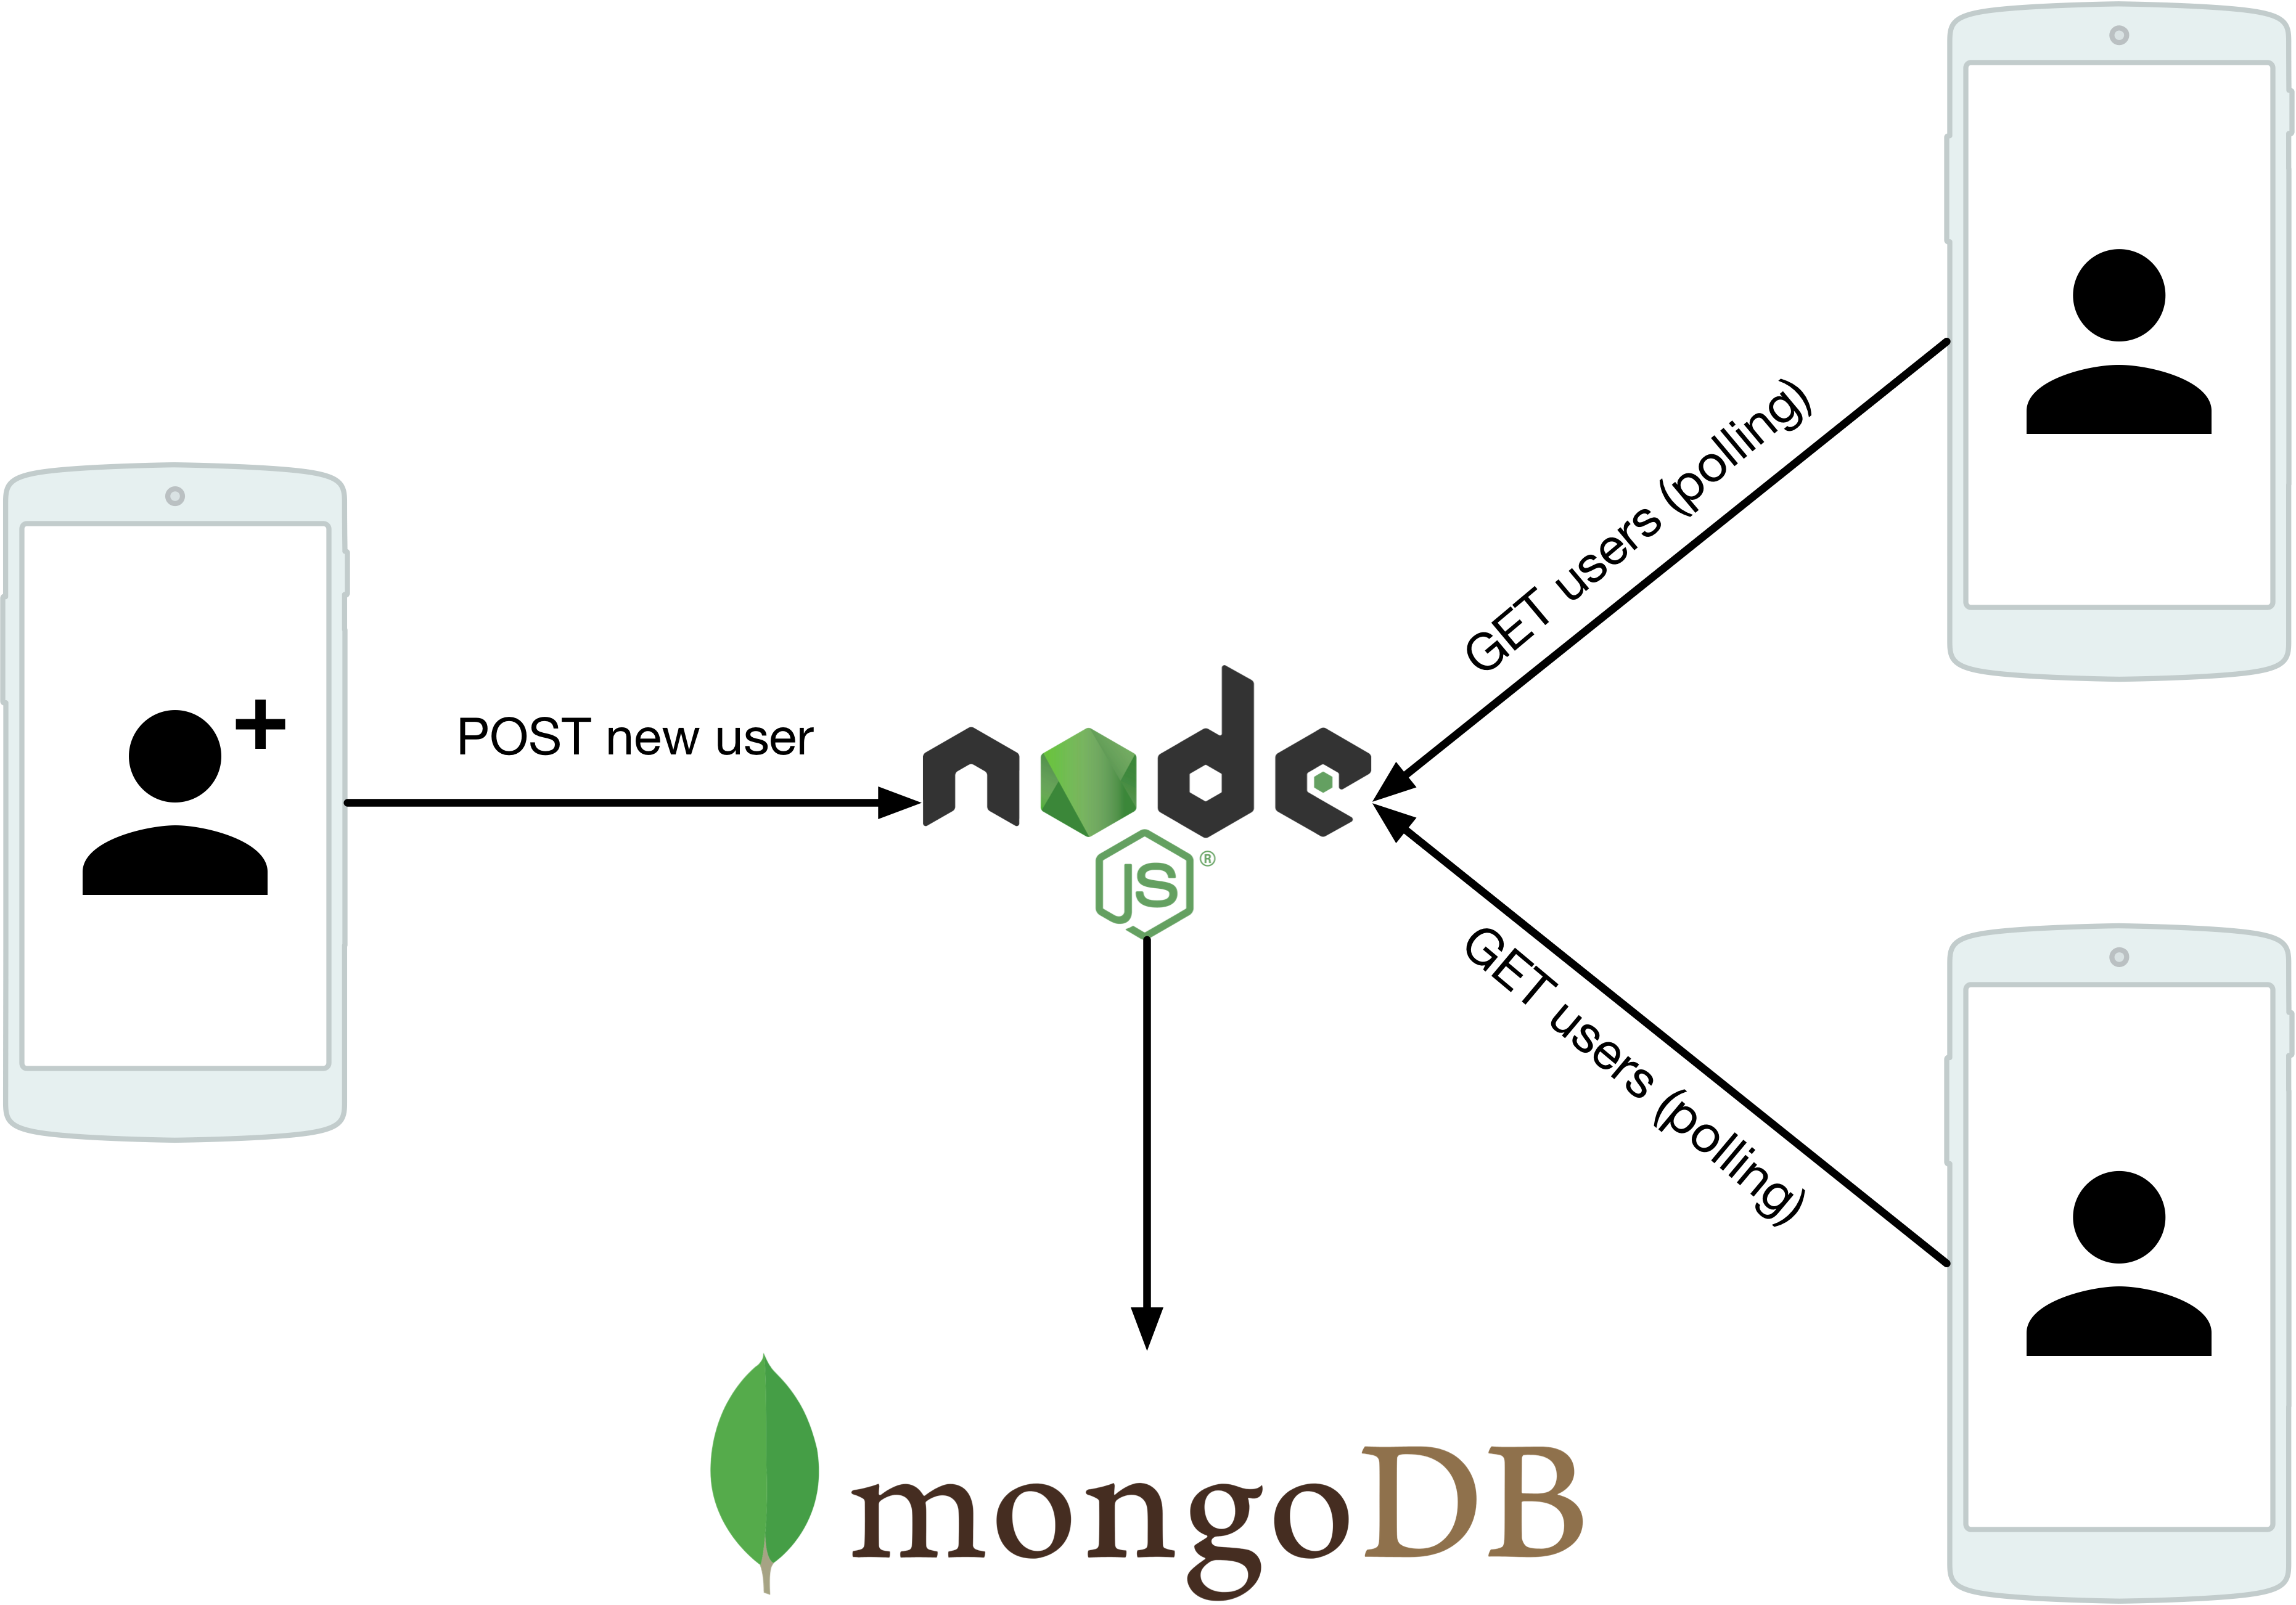
\includegraphics[width=.8\textwidth]{assets/expressmongo_architecture.png}
	\caption{Saving an object in Express/Mongo}
		\label{mongo_object_saving_figure}
\end{center}
\end{figure}
The Realm platform integrates the database directly within an object server that takes care of providing access and sending data to all the clients connected to it. This is possible thanks to the Realm runtime that you need to integrate in your client-side application and will replicate the database server on your local client.\\

On the contrary, using the Express/Mongo approach, we have the Mongo database and we built a REST API in front of it to provide access to the data. We do not need any particular runtime on the client-side and we can just handle data how we want. \\

As we can see in figures \ref{realm_object_saving_figure} and \ref{mongo_object_saving_figure}, when we create a new object on a client in Realm and save it locally, it is directly sent to the server and then pushed to other devices without needing any action. On the Express/Mongo side, you save the new object to the server and then other clients can retrieve it. \\
\paragraph{Advantages of Realm}
The advantages of Realm apply mainly on the mobile front. Realm is built to the ground up for the constrained resources and connectivity of mobile devices. It is offline first and will cache changes to be sent to the Realm server when the connection is back. Moreover, the push synchronisation of data back to the clients is the most efficient way to retrieve new data as opposed to polling data from a server at a regular interval.
\paragraph{Only for specific use cases}
The problem with Realm is that, beyond mobile, it is not very appropriate for our project. There are many pain points and small decisions that were taken by the Realm team that impose a way of doing things that may not be compatible with every project.\\

For example, one of these problems is the user authentication part and the user collection. In Realm, a user is not an object like others. It is a special object that is also used to connect to the Realm engine to handle sync. So you are limited to using Realm authentication to use the platform. Moreover, there is no way for a user with admin rights to retrieve a list of users on the client-side. This data is not accessible, unless you use the Realm Studio GUI client.\\

Another point is that, since you directly interact with the database/object server on the client-side, the code can easily be changed to access other people's information unlike a REST API where access to the database is regulated by the API. To avoid this, Realm has a system of permissions that are assigned to saved objects, but you need to assign the permissions every time you create a new object. Admins do not have direct access to everything, so you also have to add a permission for every admin every time. We wouldn't even imagine trying to add multiple set of roles here, it would be too cumbersome to handle.\\

Finally, the final point that made us abandon Realm for this project is the lack of clear solution to use it on the web. You have two ways to access the data from a web client. Either activate the GraphQL integration and write GraphQL queries to interact with the data from the web frontend. Or use the Node.JS Realm runtime to connect to the object server and serve as an API to access the data. So, even if we used Realm, we would still need to write an API. We're better off just going with the Express/Mongo option in that case. \\

It is a shame because the product provide real advantages on mobile that would take time to implement with a custom data solution, but it just isn't flexible enough and is really mobile-first while the web seems a bit like an after-thought for them. Even in their marketing material, they only present mobile-only applications such as chat or photo-sharing applications.

%%TODO add ref for Realm Studio and GraphQL explanation with footnote and ref
\subsection{Mobile application}
We needed to create a mobile client to access the information and status of a users' data from a smartphone as well as complete some administrative tasks. \\

We decided to build an Android application as well as coding the website to be responsive so it can be used on any smartphone. For the standard user, the mobile application is the one to use as it will provide access to all information, sync data offline and enable payments to other users. For the administrators, the mobile application will allow them to manage physical cards for users and for the rest of the administration, they can use the website on their smartphone.
\subsubsection{Why the need for an application?}
While we could have achieved most of the functionality with a web application, there are still some elements that require building a full mobile application. Mainly, access to device features such as NFC. With a mobile web app, we cannot have access to the NFC chip on the smartphone and thus we cannot manage physical cards or make payments through the app. This is also the reason why we only built an Android app and not an iOS one. The API for NFC on iOS\cite{apple:ios:nfc} is basic and was released in 2017, it does not allow writing on NFC tags\footnote{Unless you are a big company partnering directly with Apple} and only supported a subset of the formats of the Android API.\\

Apart from this limitation, all the other functionality could have been incorporated in a web application, for example by making a Progressive Web App (PWA). PWA are an hybrid between a mobile application and a web application and they run on desktop and mobile operating systems. Their main advantages compared to traditional web app is that they can be "installed" on the device and act like a normal application and that they generally store data offline and can sync data in the background through the user of Service Workers.
%%TODO add PWA reference
\subsubsection{Why go native?}
We could have also found a middle ground between the mobile web application and the native web application by using a mobile application framework such as Ionic or React Native to build our mobile application using web technologies. This would have allowed us to reuse some components built for the web in our mobile application.\\

We decided to opt out of that route and build our application using native Android technologies to better take advantages of the cutting-edge features announced during Google I/O 2018 \footnote{Google I/O is the annual Google developer conference held in June for developers using Google technologies (Chrome, web, Android, iOS,...)} aiming to modernise and improve the Android development workflow (see section \ref{android_chapter}).
%%TODO add ref Google I/O 2018
\subsection{Web Frontend}
Finally, we opted to use a frontend framework to provide a good structure to our client-side web application instead of relying on static custom HTML/CSS/JS.\\

The three main frameworks available at the moment are Angular\footnote{There is a distinction to be made between AngularJS (Javascript) and Angular.io (Typescript). While both coexist, you should use Angular.io as it is the version that is developed going forward. In this document, we will be talking about Angular.io when mentioning Angular}, React and Vue. \\

Vue is the youngest of the three and, while it is already growing a big community, its documentation is not as complete as the two others and its also growing rapidly which means that some of our code might become obsolete rapidly. \\

React and Angular are more mature, with Angular being the oldest of the three and are both baked by big companies: Facebook for React and Google for Angular. The biggest difference between the two is that React is Javascript-based and Angular is Typescript-based. We decided then to use Angular to take advantage of the typed nature of Typescript as well as to use Typescript for the first time in a project.

\chapter{Technologies}
\section{NFC and NDEF}
%%TODO put this in intro instead
\subsection{Introduction to NFC}
\subsection{NDEF Format}
\subsubsection{Text payload}




\section{Developing for Android}
\label{android_chapter}
Android is a mobile operating system developed by Google and launched in September 2008. The core of Android is open source and is known as the \emph{Android Open Source Program (AOSP)}. But nobody really knows or uses the AOSP version of Android, every phone manufacturer, even Google, forks the AOSP version to build its own for their devices. What is often referred as "pure Android" is the Google implementation of Android on their Nexus and Pixel lines of smartphones. Android runs on all kinds of platforms, from mobile phone to watches, as well as tablets and laptops. \\

A SDK and an IDE are provided for developing Android applications. Those applications are written mainly in Java, with the ability to write native code in C++ using the Android NDK\footnote{This is used for example to use some C++ libraries, like OpenCV.} and interact with the Java code using JNI. The support for a second language named Kotlin was announced at Google I/O 2017 (see section \ref{kotlin}). Applications run in a virtual environment on Android called ART. You can think of ART as the equivalent of the JVM for desktop Java development.
\subsection{Android Fragmentation}
One of the biggest problems for developers is the fragmentation of OS versions running on Android devices. As of May 2018, only 62.3\% of devices were running Android Marshmallow (version 6) or later. Android Marshmallow was released in 2015, meaning that 37.7\% of devices were running software that was more than 3 years old without security updates or new features (see table \ref{android_os_table}).

\begin{table}[H]
\centering
\bgroup
\def\arraystretch{1.5}%  1 is the default, change whatever you need
\begin{tabular}{|c|c|c|c|}
\hline
  \textbf{Year} & \textbf{Version Name} & \textbf{Usage of this version} & \textbf{Usage of this version or later}\\
  \hline
2010 & Gingerbread & 0.3\% & 100.0\% \\
\hline
2011 & Ice Cream Sandwich & 0.4\% & 99.7\% \\
\hline
2012 & Jelly Bean & 4.3\% & 99.3\% \\
\hline
2013 & Kit Kat & 10.3\% & 95.0\% \\
\hline
2014 & Lollipop & 22.4\% & 84.7\% \\
\hline
2015 & Marshmallow & 25.5\% & 62.3\% \\
\hline
2016 & Nougat & 31.1\% & 36.8\% \\
\hline
2017 & Oreo & 5.7\% & 5.7\% \\
\hline
\end{tabular}
\egroup
\label{android_os_table}
\caption{Android OS Fragmentation (May 2018)\cite{android:dev:osfragmentation}}
\end{table}

\subsubsection{The problem with updates}
This problem is inherent to the very nature of the Android operating system. Each phone manufacturer, or OEM, can fork its own version of Android and integrate its own skin and set of apps on top of it. When a new version of the operating system is released by Google, they can't just start using it. They have to first adapt and test all their apps and customisation with the new version before it can ship to the devices. This is a time (and by extension money) consuming process and many OEMs just don't care about maintaining their devices for more than one or two years. To make matters worse, in certain countries, such as the United States, mobile carriers have to validate and apply their own custom apps and settings on top of the OS, adding to the time needed to validate an update and causing a supplementary potential roadblock to the release of an update.

\subsubsection{What Google is doing about this?}
Google has in the recent years taken different actions to ensure that most of the devices run safe and up-to-date software on them without depending on the OEMs willingness to maintain their products.
\paragraph{Updating core apps through the Play Store}
One of the most successful changes to Android in recent years has been to slowly move all Android core applications that are present on every Android device\footnote{Actually, not every Android device. Some Asian markets, mainly China don't have access to these apps because they don't have access to any Google services. This is an edge case that won't be discussed in this document. } to the Google Play Store. These apps include for example Gmail, Google Calendar, the browser (AOSP browser and Google Chrome) and even apps like the Phone Dialer and Contacts apps. This move to the Play Store allows Google to update these applications more frequently without needing a full operating system update. While it may be seen as a necessary evil at first, because it is the only way for them to update these apps if the OEM don't apply operating system updates, it is actually a very useful move because it allows for faster iteration on these applications and quicker response for bug fixes.\\

If we compare this to the other major mobile operating system, iOS, all main applications on the platform are bundled with the OS. So, if Apple needs to update the Safari browser to support a new web API they have to release a full OS version and push it to all their devices instead of just updating the application that needs an update as Google would do on Android.
\paragraph{Android Support Library}
%% TODO Android support library
\paragraph{Project Treble}
%% TODO Project treble
\paragraph{Security updates}
%% TODO Security updates

%%TODO talk about android fragmentation, the support library naming scheme => move to AndroidX
%% Then kotlin, architecture components, abstraction of jobscheduler etc through work manager because of versions
%%TODO add NFC on Android
\subsection{Kotlin}
\label{kotlin}
As discussed in chapter \ref{android_chapter}, Kotlin has become a primary Android language in 2017. After having used this language for a first Android project last year, I decided to build all my subsequent Android application in Kotlin. The simplifications and reductions in code length provided by this language compared to Java make developing Android applications more enjoyable. It also helps avoid many runtime errors by catching many error-prone scenarios at compile time. In this section, we will go in further details in some of the advantages provided by Kotlin and how Google is encouraging developers to use Kotlin by introducing new Kotlin-specific features in the Android SDK.
\subsubsection{Full interoperability with Java}
\subsubsection{Data classes}
Java is often defined by its detractors as a very verbose language, requiring to write a lot of repetitive boilerplate code\footnote{Boilerplate code or boilerplate refers to sections of code that have to be included in many places with little or no alteration\cite{wiki:define:boilerplate}} for simple tasks. One of these tasks is the creation of classes with accessors and mutators for some of the class fields and overriding \verb+equals+ and \verb+toString+ methods. In Object Oriented Programming, we often have to write a lot of small classes just to match the Models in our applications. These are often referred as Beans or POJOs\footnote{Plain Old Java Object}. Kotlin introduces the concept of data classes\cite{kotlin:doc:data_classes} to simplify the implementation of these type of classes. By using a data class, you get "for free" an accessor (and mutator) for each field of the class, a correct overriding of the \verb+equals+ method, an overriding of the \verb+toString+ method listing the values of all fields in the instance and a \verb+copy+ method corresponding to a copy constructor in Java. For example, if we take a simple person class in Java:
\javacode{assets/code/java/Person.java}
And then the same class written using data classes in Kotlin:
\kotlincode{assets/code/kotlin/Person.kt}
\subsubsection{Constants first}
\subsubsection{Class extensions}
\subsubsection{Null safety}

%%TODO: Good points about Kotlin:
%% - Lifting return/assignments from try/catch blocks => assignment to constants instead of empty variable first to guarantee default value
%% - Class extensions => often calling a static method of an helper class in a method-like syntax for the current class => "0.0".toDouble() instead of Double("0.0")
\subsubsection{Android KTX}
\subsection{Android Jetpack}
%%TODO talk about former name, goal was to provide a set of "good behaviors" etc
\subsubsection{Room - Data persistence}
\begin{figure}[H]
\begin{center}
	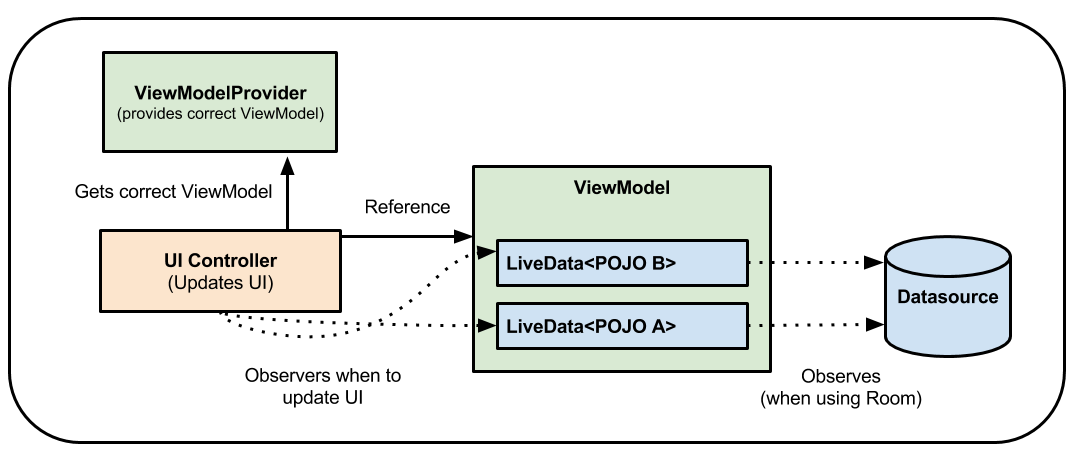
\includegraphics[width=.8\textwidth]{assets/viewmodel}
	\caption{View model interactions\cite{android:doc:viewmodel}}
\end{center}
\end{figure}
\paragraph{VieModel}
\paragraph{LiveData}
%%TODO talk about lifecycle observers and lifecycle aware

\subsubsection{Work Manager - Background jobs}
\subsubsection{Navigation}

\section{NoSQL Database - MongoDB}
\subsection{Storage as JSON/BSON documents}
%%TODO verify this is true
\subsection{How to handle references}
\label{mongo_references}
%%TODO add source on mongo site https://docs.mongodb.com/manual/applications/data-models-relationships/
%%TODO talk about embedding documents vs ids of childrens vs ids of parent for different sizes
\subsection{Mongoose}

\subsubsection{Schemas}
\subsubsection{Promises with Mongoose}
%%TODO find function, insert etc with await => talk about command than talk directly to mongo without passing by mongoose
\subsubsection{Populating references}
\subsubsection{Hooks}
\label{mongoose_hooks}
%%TODO talk about pre('remove') for example
\section{NodeJS et Express}
\subsection{JavaScript ES6}
\subsection{NPM Modules}
\subsection{Promises}
\subsection{Middlewares}
\subsection{PassportJS}

\section{Angular 6}
%%runs with npm, talk about ng-cli and generation etc of component 
\subsection{Single-page webapp}
\subsection{Dependencies injection}
\subsection{Architecture of an Angular Application}
\begin{figure}[H]
\begin{center}
	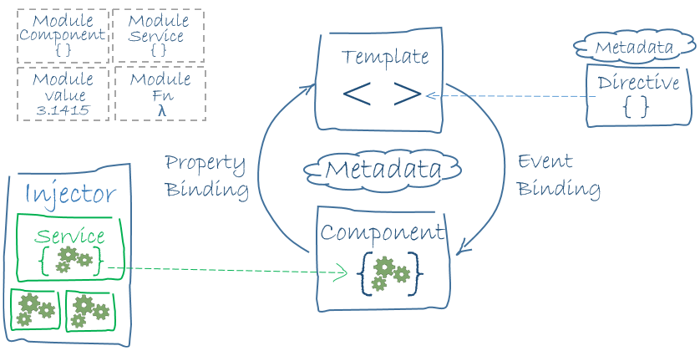
\includegraphics[width=.8\textwidth]{assets/angular_architecture}
	\caption{Architecture of an Angular application\cite{angular:ref:architecture}}
\end{center}
\end{figure}
\subsubsection{Components}
\paragraph{Templates}
\paragraph{Communication between components - Input/Output}
\subsubsection{Services}
\subsubsection{Routing and Guards}
\subsection{RxJS - Observables}
\subsection{Reactive Forms}
\subsection{TypeScript}
\subsection{Angular Material}

\section{Containers - Infrastructure as code}
\subsection{Docker}
\subsection{Orchestration avec Docker Compose}
\subsection{Google Cloud}
\subsubsection{Kubernetes}
\subsubsection{Google Container Registry}
\subsection{Azure}

\chapter{Implémentation}
\section{Modules du projet}
\section{Déploiement}
\subsection{Architecture du projet}
\subsection{Proxy Nginx}
\section{Le backend commun}
\subsection{Authentification}
\subsection{Endpoints}
\subsection{Interaction avec la base de données}
\section{Le frontend Angular}
\subsection{Routing}
\subsection{Components}
\chapter{Résultats}
\chapter{Conclusion}
%%TODO talk about how to implement new features or sections inside the project
\section{Future works}
\bibliographystyle{unsrt}
\bibliography{bibliography}

\end{document}
